\documentclass{presentation}
\newcommand{\wbf}{\mathbf{w}}
\newcommand{\Wbf}{\mathbf{W}}
\newcommand{\xbf}{\ensuremath{\mathbf{x}}}
\newcommand{\zbf}{\ensuremath{\mathbf{z}}}
\newcommand{\zerobf}{\mathbf{0}}
\newcommand{\h}{h}
\newcommand{\dist}{\mathrm{dist}}

\newcommand{\Acal}{\ensuremath{\mathcal{A}}}
\newcommand{\Bcal}{\ensuremath{\mathcal{B}}}
\newcommand{\Ccal}{\ensuremath{\mathcal{C}}}
\newcommand{\Dcal}{\ensuremath{\mathcal{D}}}
\newcommand{\Fcal}{\ensuremath{\mathcal{F}}}
\newcommand{\Hcal}{\ensuremath{\mathcal{H}}}
\newcommand{\Mcal}{\ensuremath{\mathcal{M}}}
\newcommand{\Ncal}{\ensuremath{\mathcal{N}}}
\newcommand{\Pcal}{\ensuremath{\mathcal{P}}}
\newcommand{\Scal}{\ensuremath{\mathcal{S}}}
\newcommand{\Tcal}{\ensuremath{\mathcal{T}}}
\newcommand{\Xcal}{\ensuremath{\mathcal{X}}}
\newcommand{\Ycal}{\ensuremath{\mathcal{Y}}}
\newcommand{\Zcal}{\ensuremath{\mathcal{Z}}}

\newcommand{\Ebb}{\ensuremath{\mathbb{E}}}
\newcommand{\Pbb}{\ensuremath{\mathbb{P}}}
\newcommand{\Rbb}{\ensuremath{\mathbb{R}}}
\newcommand{\Nbb}{\ensuremath{\mathbb{N}}}

\newcommand{\Rfrak}{\ensuremath{\mathfrak{R}}}

\newcommand{\RA}{\right\rangle}
\newcommand{\LA}{\left\langle}
\newcommand{\LB}{\left[}
\newcommand{\RB}{\right]}
\newcommand{\LC}{\left\{}
\newcommand{\LM}{\left\|}
\newcommand{\RM}{\right\|}
%\newcommand{\RC}{\right\}}
%\newcommand{\RN}{\right\vert}
\newcommand{\LN}{\left\vert}
\newcommand{\LP}{\left(}
\newcommand{\RP}{\right)}

\newcommand{\wrt}{{\it w.r.t.}\xspace}
\newcommand{\eg}{{\it e.g.}\xspace}
\newcommand{\ie}{{\it i.e.}\xspace}
\newcommand{\iid}{{\it i.i.d.}\xspace}

\newcommand{\defeq}{:=}

\DeclareMathOperator*{\EE}{\Ebb}
\DeclareMathOperator*{\PP}{\Pbb}
\DeclareMathOperator*{\argmin}{\mathrm{argmin}}
\DeclareMathOperator*{\vect}{\mathrm{vec}}
\DeclareMathOperator*{\leaky}{\mathrm{Leaky}}
\DeclareMathOperator*{\proj}{\mathrm{Proj}}

\newcommand{\Irm}{\mathrm{I}}
\newcommand{\KL}{\mathrm{KL}}
\newcommand{\KLr}{\overline{\KL}}
\newcommand{\Hell}{H^2}
\newcommand{\TV}{TV}
\newcommand{\kl}{\mathrm{kl}}
\newcommand{\W}{\mathrm{W}}
\newcommand{\Lip}{\mathrm{Lip}}

\newcommand{\D}{\Dcal}
\newcommand{\Dm}{\Dcal_{m}}
\renewcommand{\H}{\Hcal}
\newcommand{\Hb}{\overline{\Hcal}}
\newcommand{\loss}{\ell}
\renewcommand{\P}{\mathrm{P}}
\newcommand{\Q}{\mathrm{Q}}
\newcommand{\R}{\Rbb}
\newcommand{\N}{\Nbb}
\renewcommand{\S}{\Scal}
\newcommand{\Sm}{\S_m}
\newcommand{\Risk}{\text{R}}
\newcommand{\Riskhat}{\hat{\Risk}}
\newcommand{\X}{\Xcal}
\newcommand{\x}{\xbf}
\newcommand{\y}{y}
\newcommand{\Y}{\Ycal}
\newcommand{\Z}{\Zcal}
\newcommand{\z}{\zbf}
\newcommand{\varepsilonbf}{\boldsymbol{\varepsilon}}
\newcommand{\rad}{\mathdbcal{E}}
\newcommand{\DS}{\D_\S}
\newcommand{\yeast}{{\sc Yeast}\xspace}
\newcommand{\phishing}{{\sc Phishing}\xspace}
\newcommand{\mushrooms}{{\sc Mushrooms}\xspace}
\newcommand{\mnist}{{\sc MNIST}\xspace}
\newcommand{\fashion}{{\sc FashionMNIST}\xspace}
\newcommand{\indic}{\mathds{1}}

\newcommand{\OPBTest}{\normalfont\textsc{OPBTest} }
\newcommand{\OPBTrain}{\normalfont\textsc{OPBTrain} }

\newcommand{\Vhat}{\hat{V}}
\newcommand{\Bhat}{\hat{B}}
\DeclareMathOperator*{\ReLU}{\mathrm{ReLU}}

\newcommand{\Cfrak}{\ensuremath{\mathfrak{C}}}

\newcommand{\Poinc}{\texttt{Poinc}}
\newcommand{\Lsob}{\texttt{L-Sob}}
\newcommand{\Ent}{\mathrm{Ent}}
\newcommand{\Var}{\mathrm{Var}}
\DeclareMathOperator*{\Err}{\mathrm{Err}}


\let\oldQ\Q
\let\oldP\P
\renewcommand{\Q}{\orange{\oldQ}}
\renewcommand{\P}{\green{\oldP}}


%%\setbeameroption{show notes}
%\setbeameroption{show notes on second screen=right}


\title{PAC-Bayes Learning From\\ an Optimisation Perspective}
\subtitle{Soutenance de doctorat}

\author{\vspace{-1.5cm}
 Maxime Haddouche}
 
\institute{
\vspace{1.8cm}
Inria London\\
Université de Lille\\
}

\date{\vspace{0.5cm}

{\bf Mercredi 2 Octobre 2024}}

\begin{document}

%%%%%%%%%%%%%%%%%%%%%%%%%%%%%%%%%%%%%%%%%%%%%%%%%%%%%%%%%%%%%%%%%%%%%%%%%%%%%%%
%TODO Logo Lille et Inria London
\begin{xframe}{}
    \maketitle
\end{xframe}


\begin{xframe}{Summary}
    \tableofcontents
\end{xframe}

\section{Overwiew of the PhD}
%TODO General introduction on PhD, Inria London, Collaborators, research projects in and out the manuscript

\section{Introduction to PAC-Bayes Learning}
%Keep those two slides, + detail Catoni, McAllester bound and associated algorithms + biblio
%Also detail the two diagrams to explain the goal of the PhD
%At the beginning of each part, detail which part of the diagram we are investigating 



   \begin{xframe}{What is PAC-Bayes ?}

    \vspace{-0.2cm}
    \textbf{Learning theory goal:} Learn the best $h\in\H$ to answer a given problem
    \begin{block}{\bf PAC-Bayes: Find the best distribution over $\H$ ! }
    Learning a posterior $\Q$ over models from $m$ data and a prior distribution $\P$
    \end{block}
    
    \vspace{-0.2cm}
    
    \begin{figure}
      \includestandalone[width=0.8\linewidth]{figures/intro}
    \end{figure}
    
    \vspace{-0.6cm}
    \uncover<2->{
    \begin{block}{}
    {\bf PAC-Bayesian generalisation bounds in a nutshell}\\[0.0cm]
    {\footnotesize With probability at least $1-\delta$}\\[-0.7cm]
    \begin{align*}
    \text{performance gap}(\Q) \le \text{bound}\Big(\text{complexity}(\Q, \P), \tfrac{1}{m}, \ln\tfrac{1}{\delta}\Big)
    \end{align*}
    \vspace{-0.7cm}
    \end{block}}

    {\tiny Image from Paul Viallard. }
    \end{xframe}

    \begin{xframe}{Setting}

        \vfill
      
        \xscalebox{1}{
        {\bf Notations:}
        \begin{xitemize}
            \item Predictor/hypothesis $h\in\H$, Data space $\mathcal{Z}$
            \item Loss $\ell: \Hcal\times\Zcal\to \Rbb$, 
            \item Countable learning sample $\S= (\z_i)_{i\geq 1}\in\mathcal{Z}^\Nbb$,  with distribution $\displaystyle \DS$ 
            \item $\displaystyle \Sm$:  Restriction of $\S$ to  $m$ first points with distribution $\Dm$
            \item Space of distributions over $\mathcal{H}$: $\Mcal(\H)$
            \item Posterior and prior distribution $\Q,\P\in\Mcal(\H)^2$
            \item If $\Sm\sim\D^{m}$ \iid, Risks: $\Risk_{\D}(h)=\EE_{\z\sim\D}\loss(h, \z)$, $\Riskhat_{\Sm}(h)=\frac{1}{m}\sum_{i=1}^{m}\loss(h, \z_i)$
            \item Expected risks $\Risk_{\D}(\Q) = \displaystyle\EE_{h\sim\Q}[\Risk_{\D}(h)],$ \hspace{0.1cm} $\Riskhat_{\Sm}(\Q) = \displaystyle\EE_{h\sim\Q}[\Riskhat_{\S}(h)]$
            \end{xitemize}
        }
       
       \end{xframe}

\begin{xframe}{\bf Two classical bounds}

    \begin{block}{{\bf McAllester's bound (Maurer's improvement) \citet[Theorem 5]{Maurer2004}}~{\small ($\ell\in[0,1]$)}}
        For any $\P\in\Mcal(\H)$, with probability $1{-}\delta$ over $\Sm\sim\Dcal^m$, for any $\Q\in \Mcal(\Hcal)$,
       $$\Risk_{\D}(\Q) \le \Riskhat_{\S}(\Q)+\sqrt{\frac{\KL(\Q,\P)+\ln\frac{2\sqrt{m}}{\delta}}{2m}}$$
     \end{block}

    \begin{block}{{\bf Catoni's bound \citet[Theorem 4.1]{AlquierRidgwayChopin2016}}~{\small ($\ell$ $\sigma$-subgaussian)}}
        For $\lambda>0$, $\P\in\Mcal(\H)$, with probability $1{-}\delta$ over $\Sm\sim\Dcal^m$, for any $\Q\in \Mcal(\Hcal)$,
       $$\Risk_{\D}(\Q) \le \Riskhat_{\S}(\Q)+\frac{\KL(\Q,\P)+\ln\frac{1}{\delta}}{\lambda} + \frac{\lambda\sigma^2}{2m}$$
     \end{block}
\end{xframe}
 
\begin{xframe}{From bounds to algorithms}
    \textbf{Previous bounds:} both fully empirical $\rightarrow$ optimisation in $\Q$ is feasible on $\mathcal{C}\subseteq \Mcal(\Hcal)$ ! 
    \begin{align*}
        \text{McAllester} \hspace{0.5cm} &\Q_{M}:= \underset{\Q\in\mathcal{C}}{\operatorname{argmin}}\; \Riskhat_{\Sm}(\Q) + \sqrt{\frac{\KL(\Q,\P)}{2m}}.
        \intertext{For any $\lambda>0$,}
        \text{Catoni}\hspace{0.5cm} &\Q_{C}:= \underset{\Q\in\mathcal{C}}{\operatorname{argmin}}\; \Riskhat_{\Sm}(\Q) +\frac{\KL(\Q,\P)}{\lambda}.
      \end{align*}

    If $\mathcal{C}= \Mcal(\Hcal)$, a \emph{Gibbs posterior} $\P_{-\lambda \Riskhat_{\Sm}}$ is the explicit minimiser of Catoni's bound:

    \begin{align*}
        d\P_{-\lambda \Riskhat_{\Sm}}(h) = \frac{\exp(-\lambda \Riskhat_{\Sm}(h))}{\Ebb_{h\sim\P}[\exp(-\lambda \Riskhat_{\Sm}(h))]} d\P(h)
    \end{align*}
\end{xframe}

\begin{xframe}{Practical instantiation}
    \begin{block}{\bf Quick sum up}
        PAC-Bayes algorithms minimise theoretical bounds $\rightarrow$ sound theoretical guarantees comes with our posterior. 
    \end{block}
    \textbf{Drawbacks} Often hard to optimise on $\Mcal(\Hcal)$, and Gibbs posterior implementation is time-consuming. 

    \uncover<2->{ 
        \begin{block}{\bf Questions}
            \begin{enumerate}
                \item How are those algorithms instantiated in practice?
                \item Are these algorithms efficient and do they come with non-vacuous theoretical guarantees? %add the fact that there is fast-rate pac bayes bounds
              \end{enumerate}
        \end{block}

    }
\end{xframe}


\begin{xframe}{To sum up: PAC-Bayes Through Information Theory }
    \begin{figure}
        \centering
        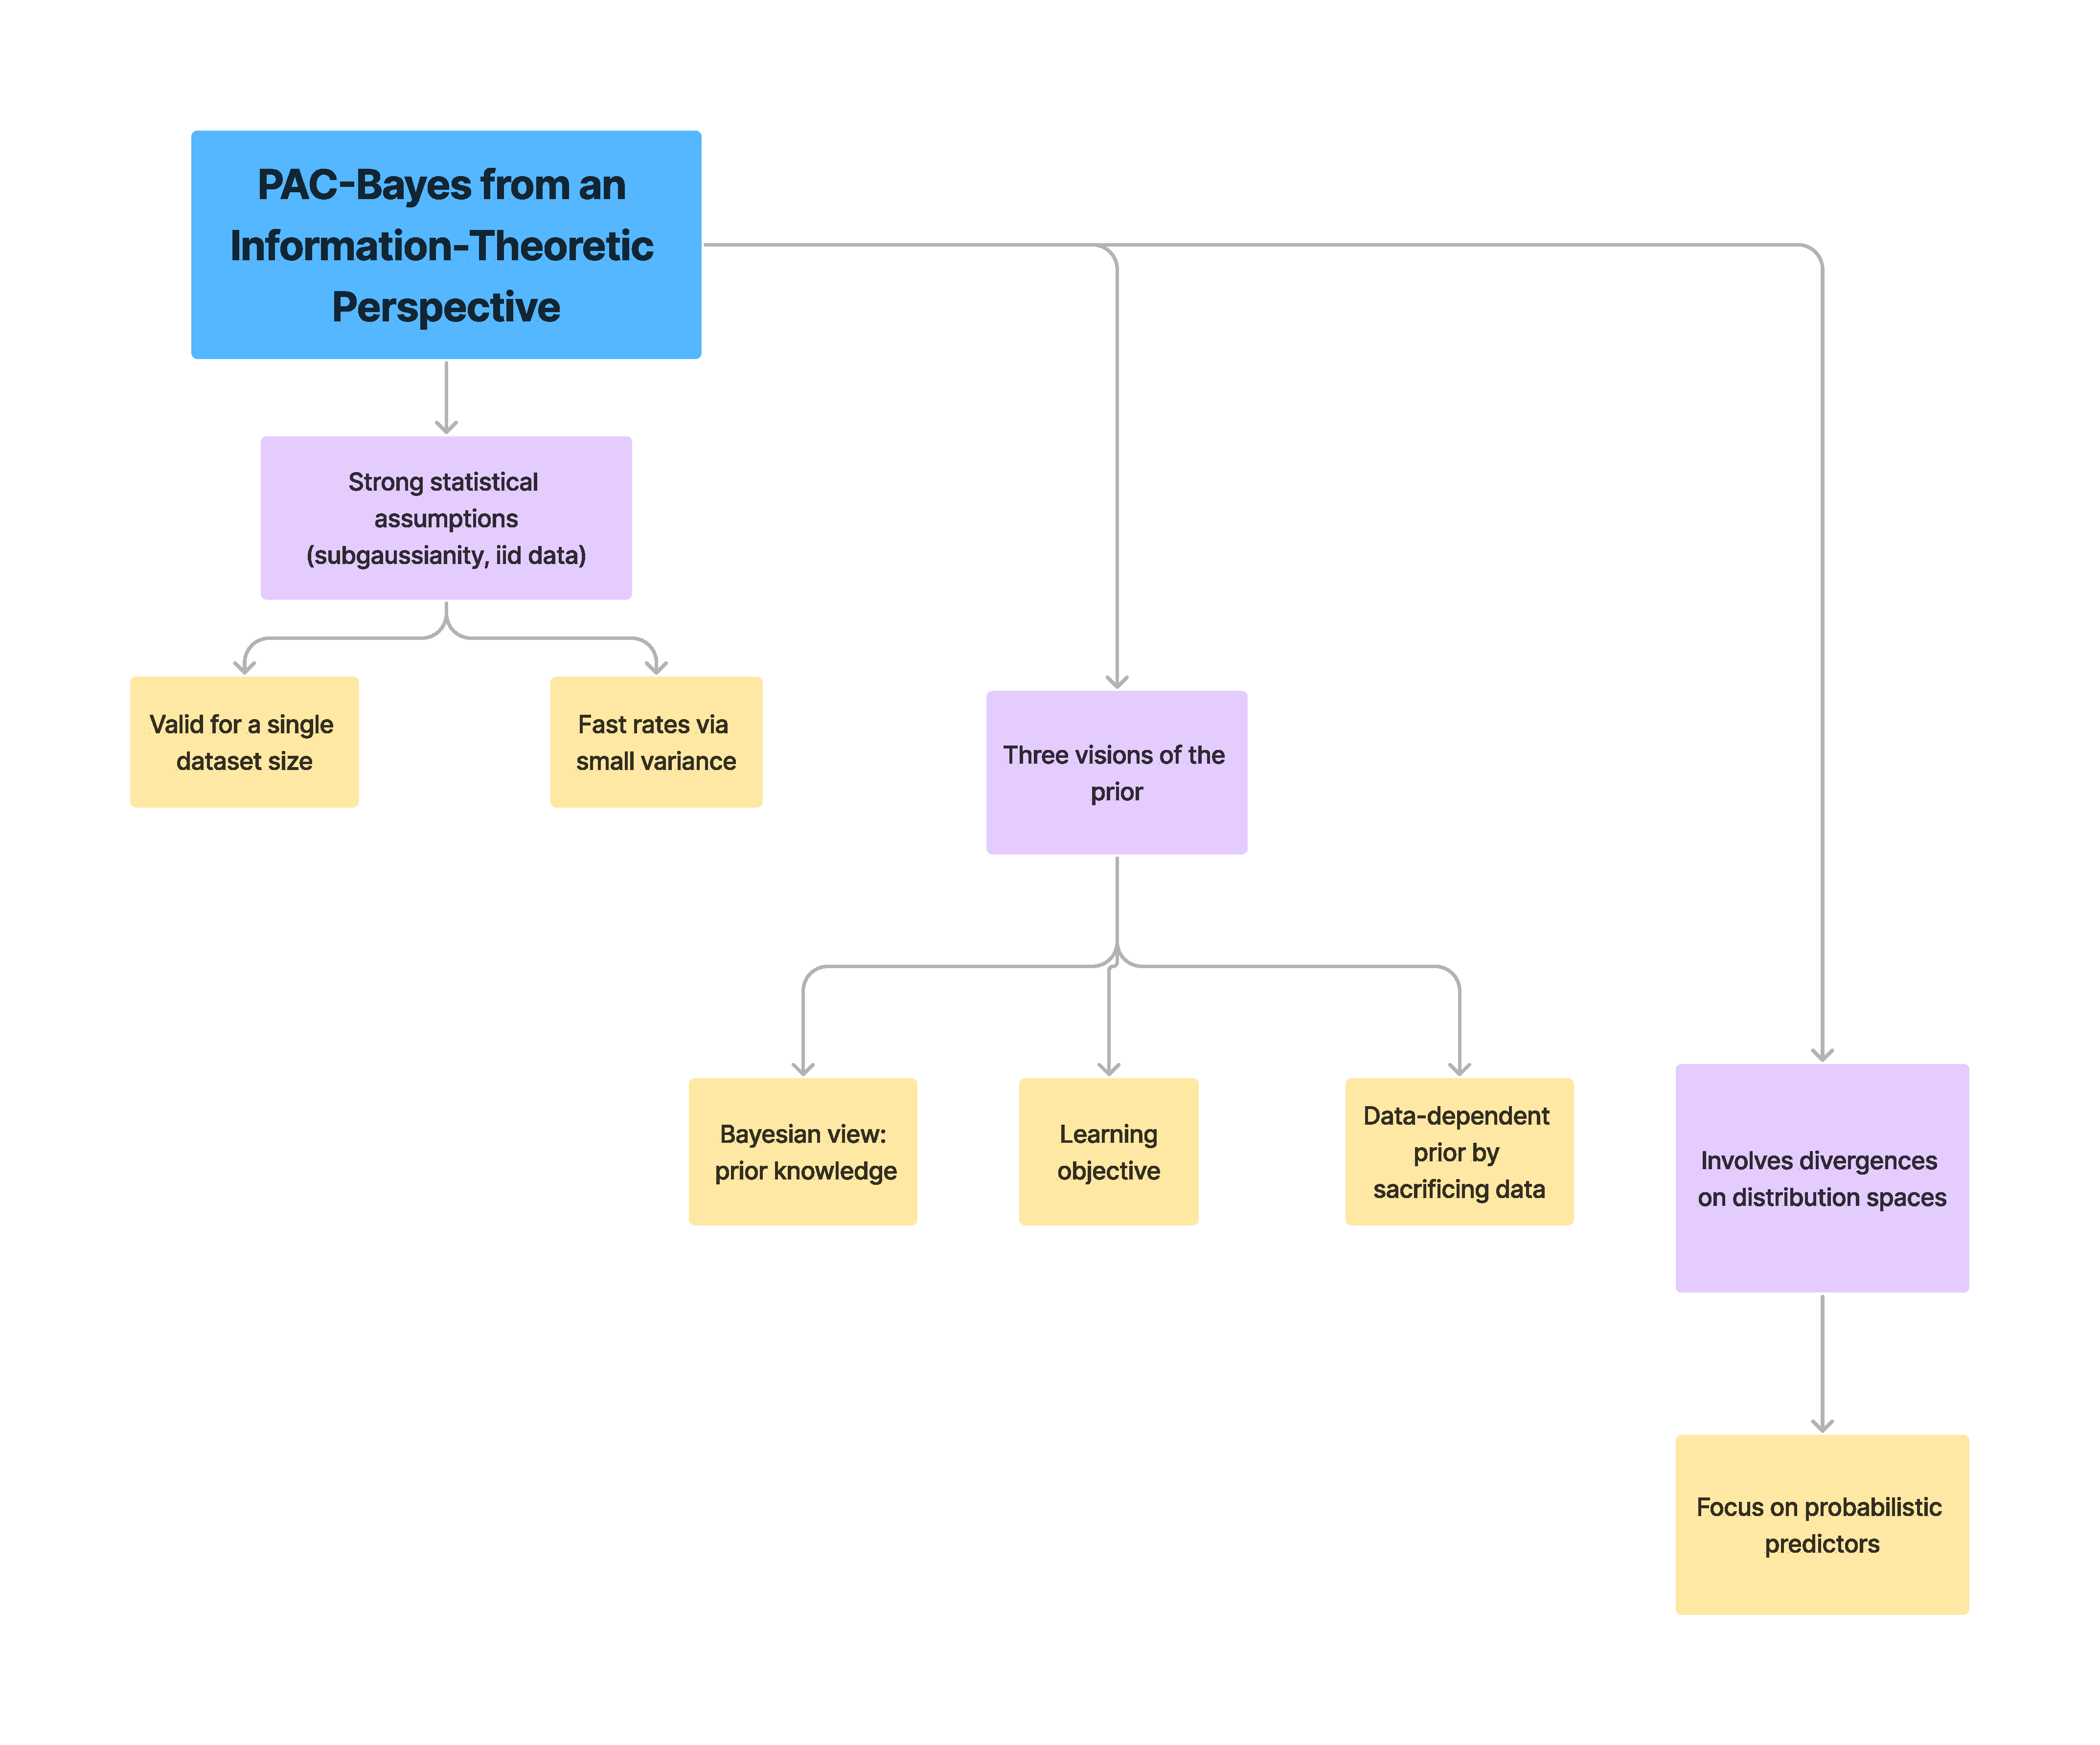
\includegraphics[scale=0.14]{recap-info.pdf}
    \end{figure}
  \end{xframe}

  \begin{xframe}{Contribution: PAC-Bayes with an Optimisation Perspective }
    \begin{figure}
        \centering
        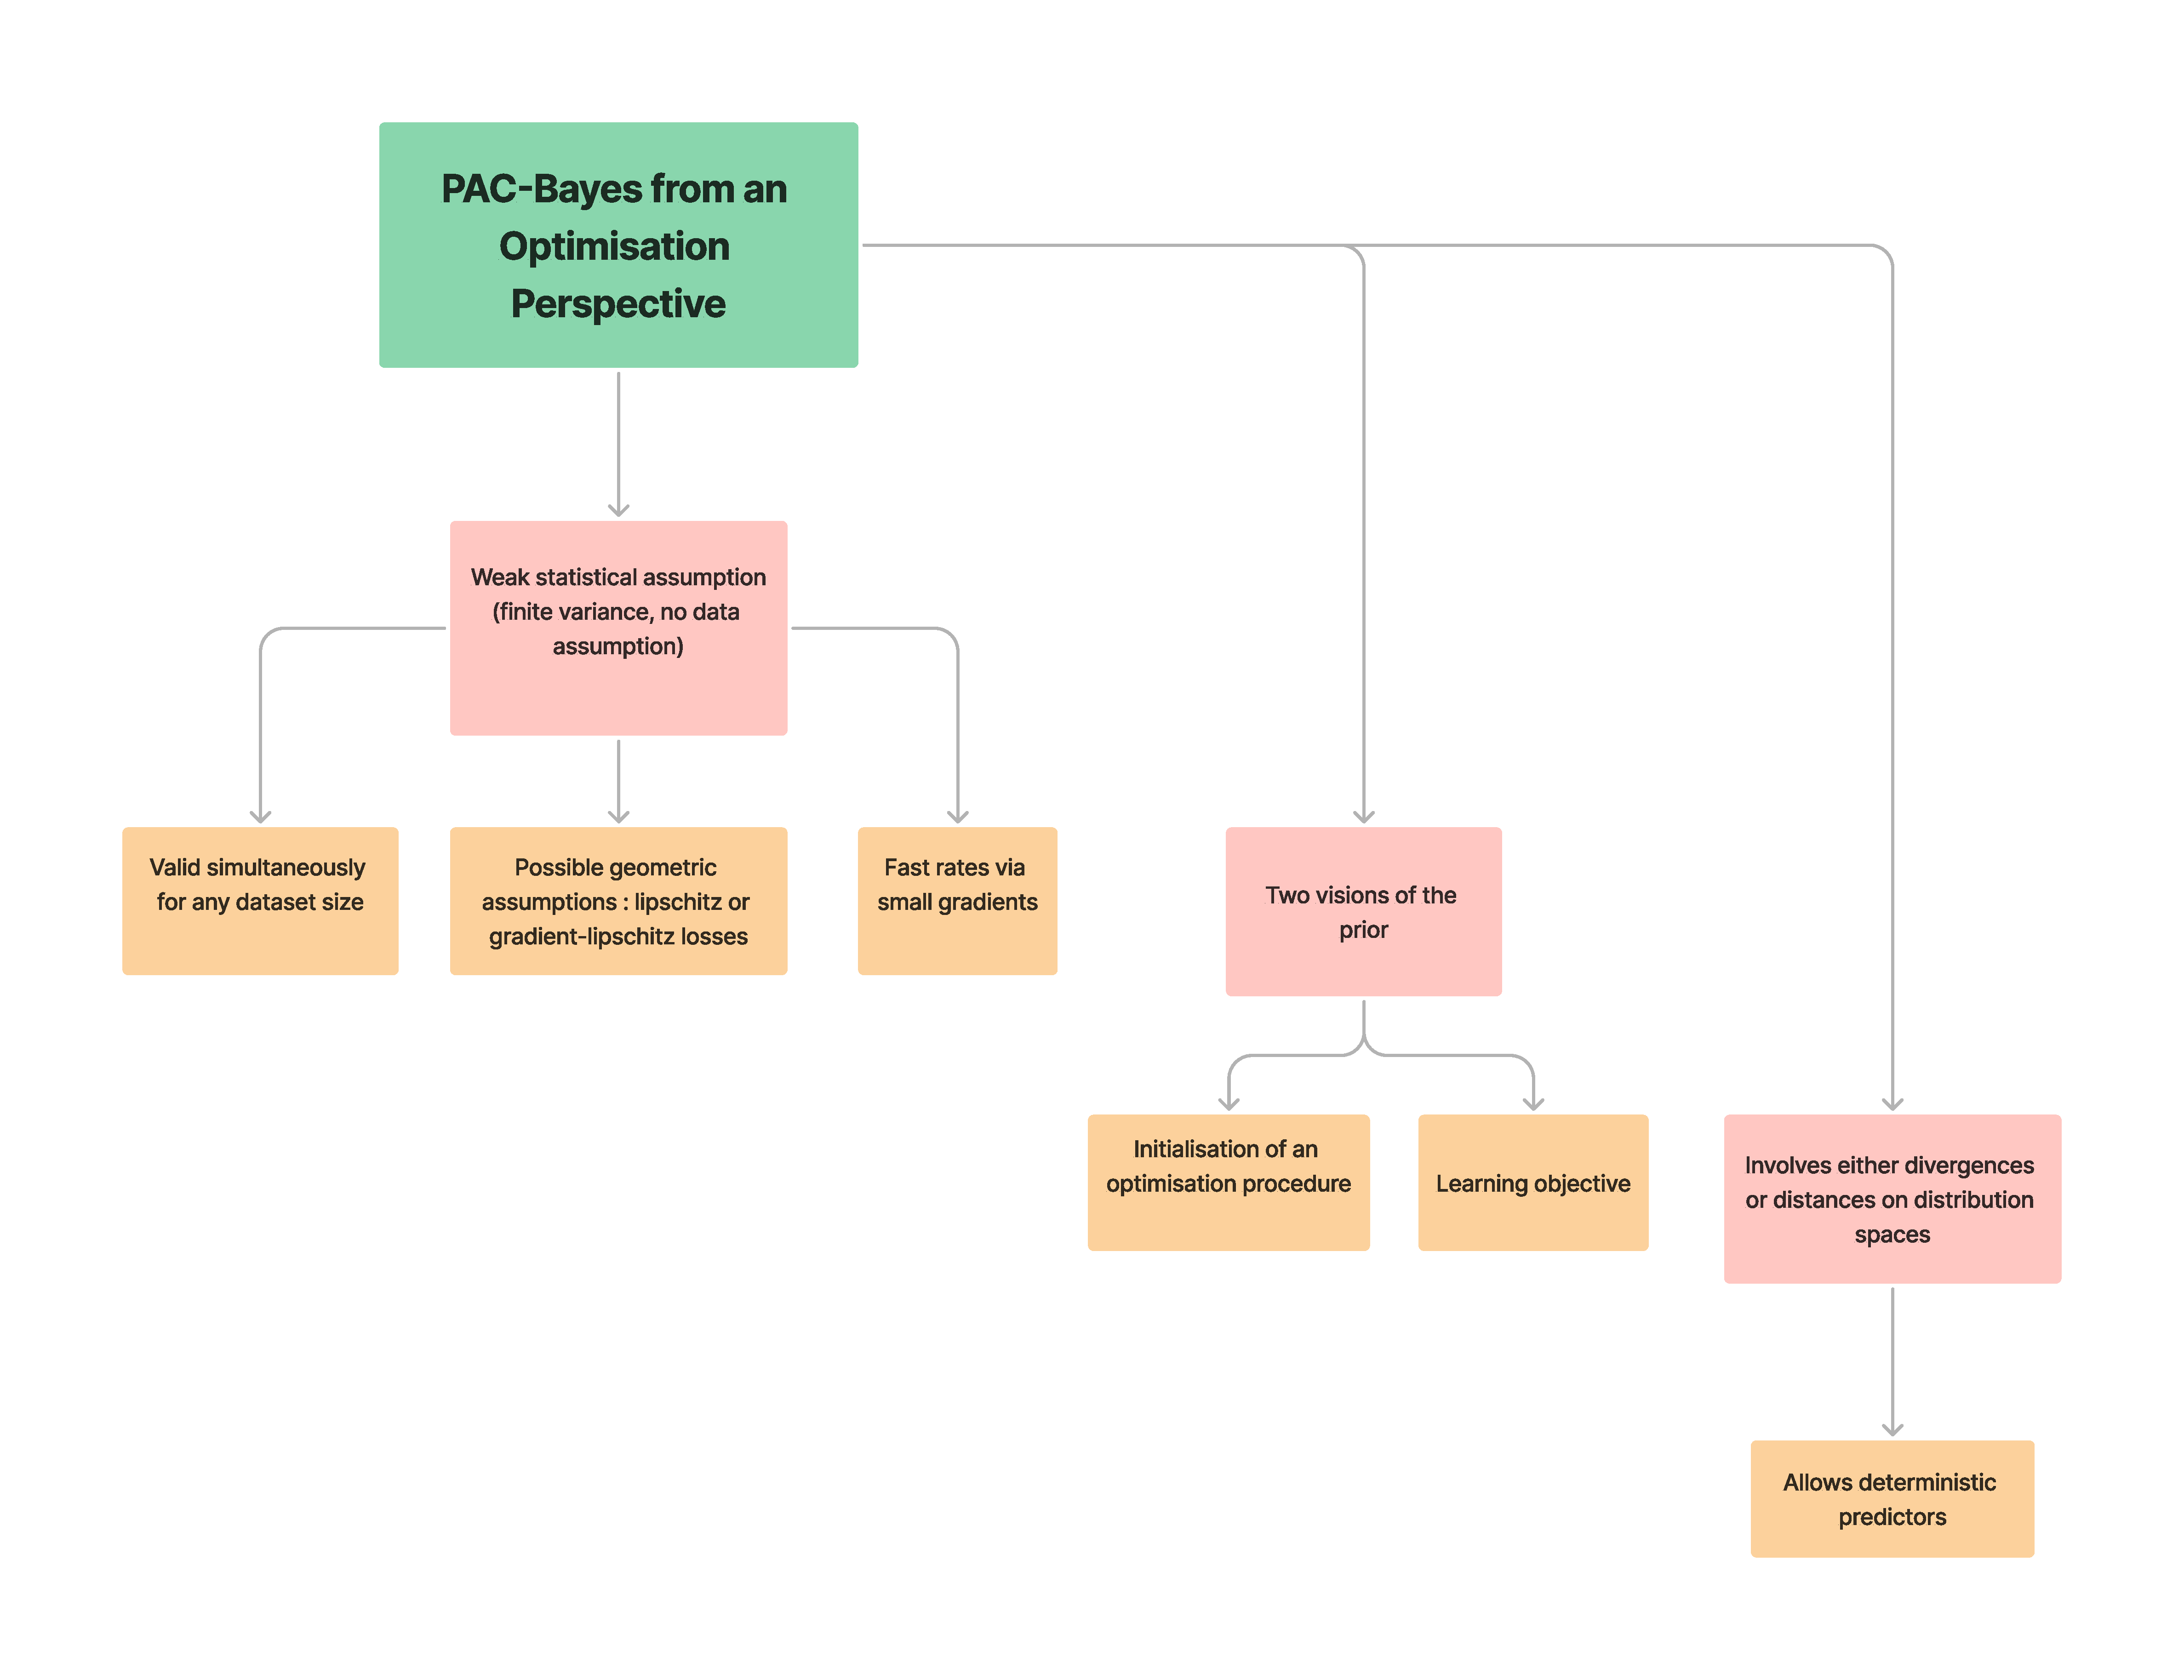
\includegraphics[scale=0.14]{recap-optim.pdf}
    \end{figure}
  \end{xframe}


\section{PAC-Bayes with Weak Statistical Assumptions}

\begin{xframe}{PAC-Bayes with Weak Statistical Assumptions}
  \begin{figure}
      \centering
      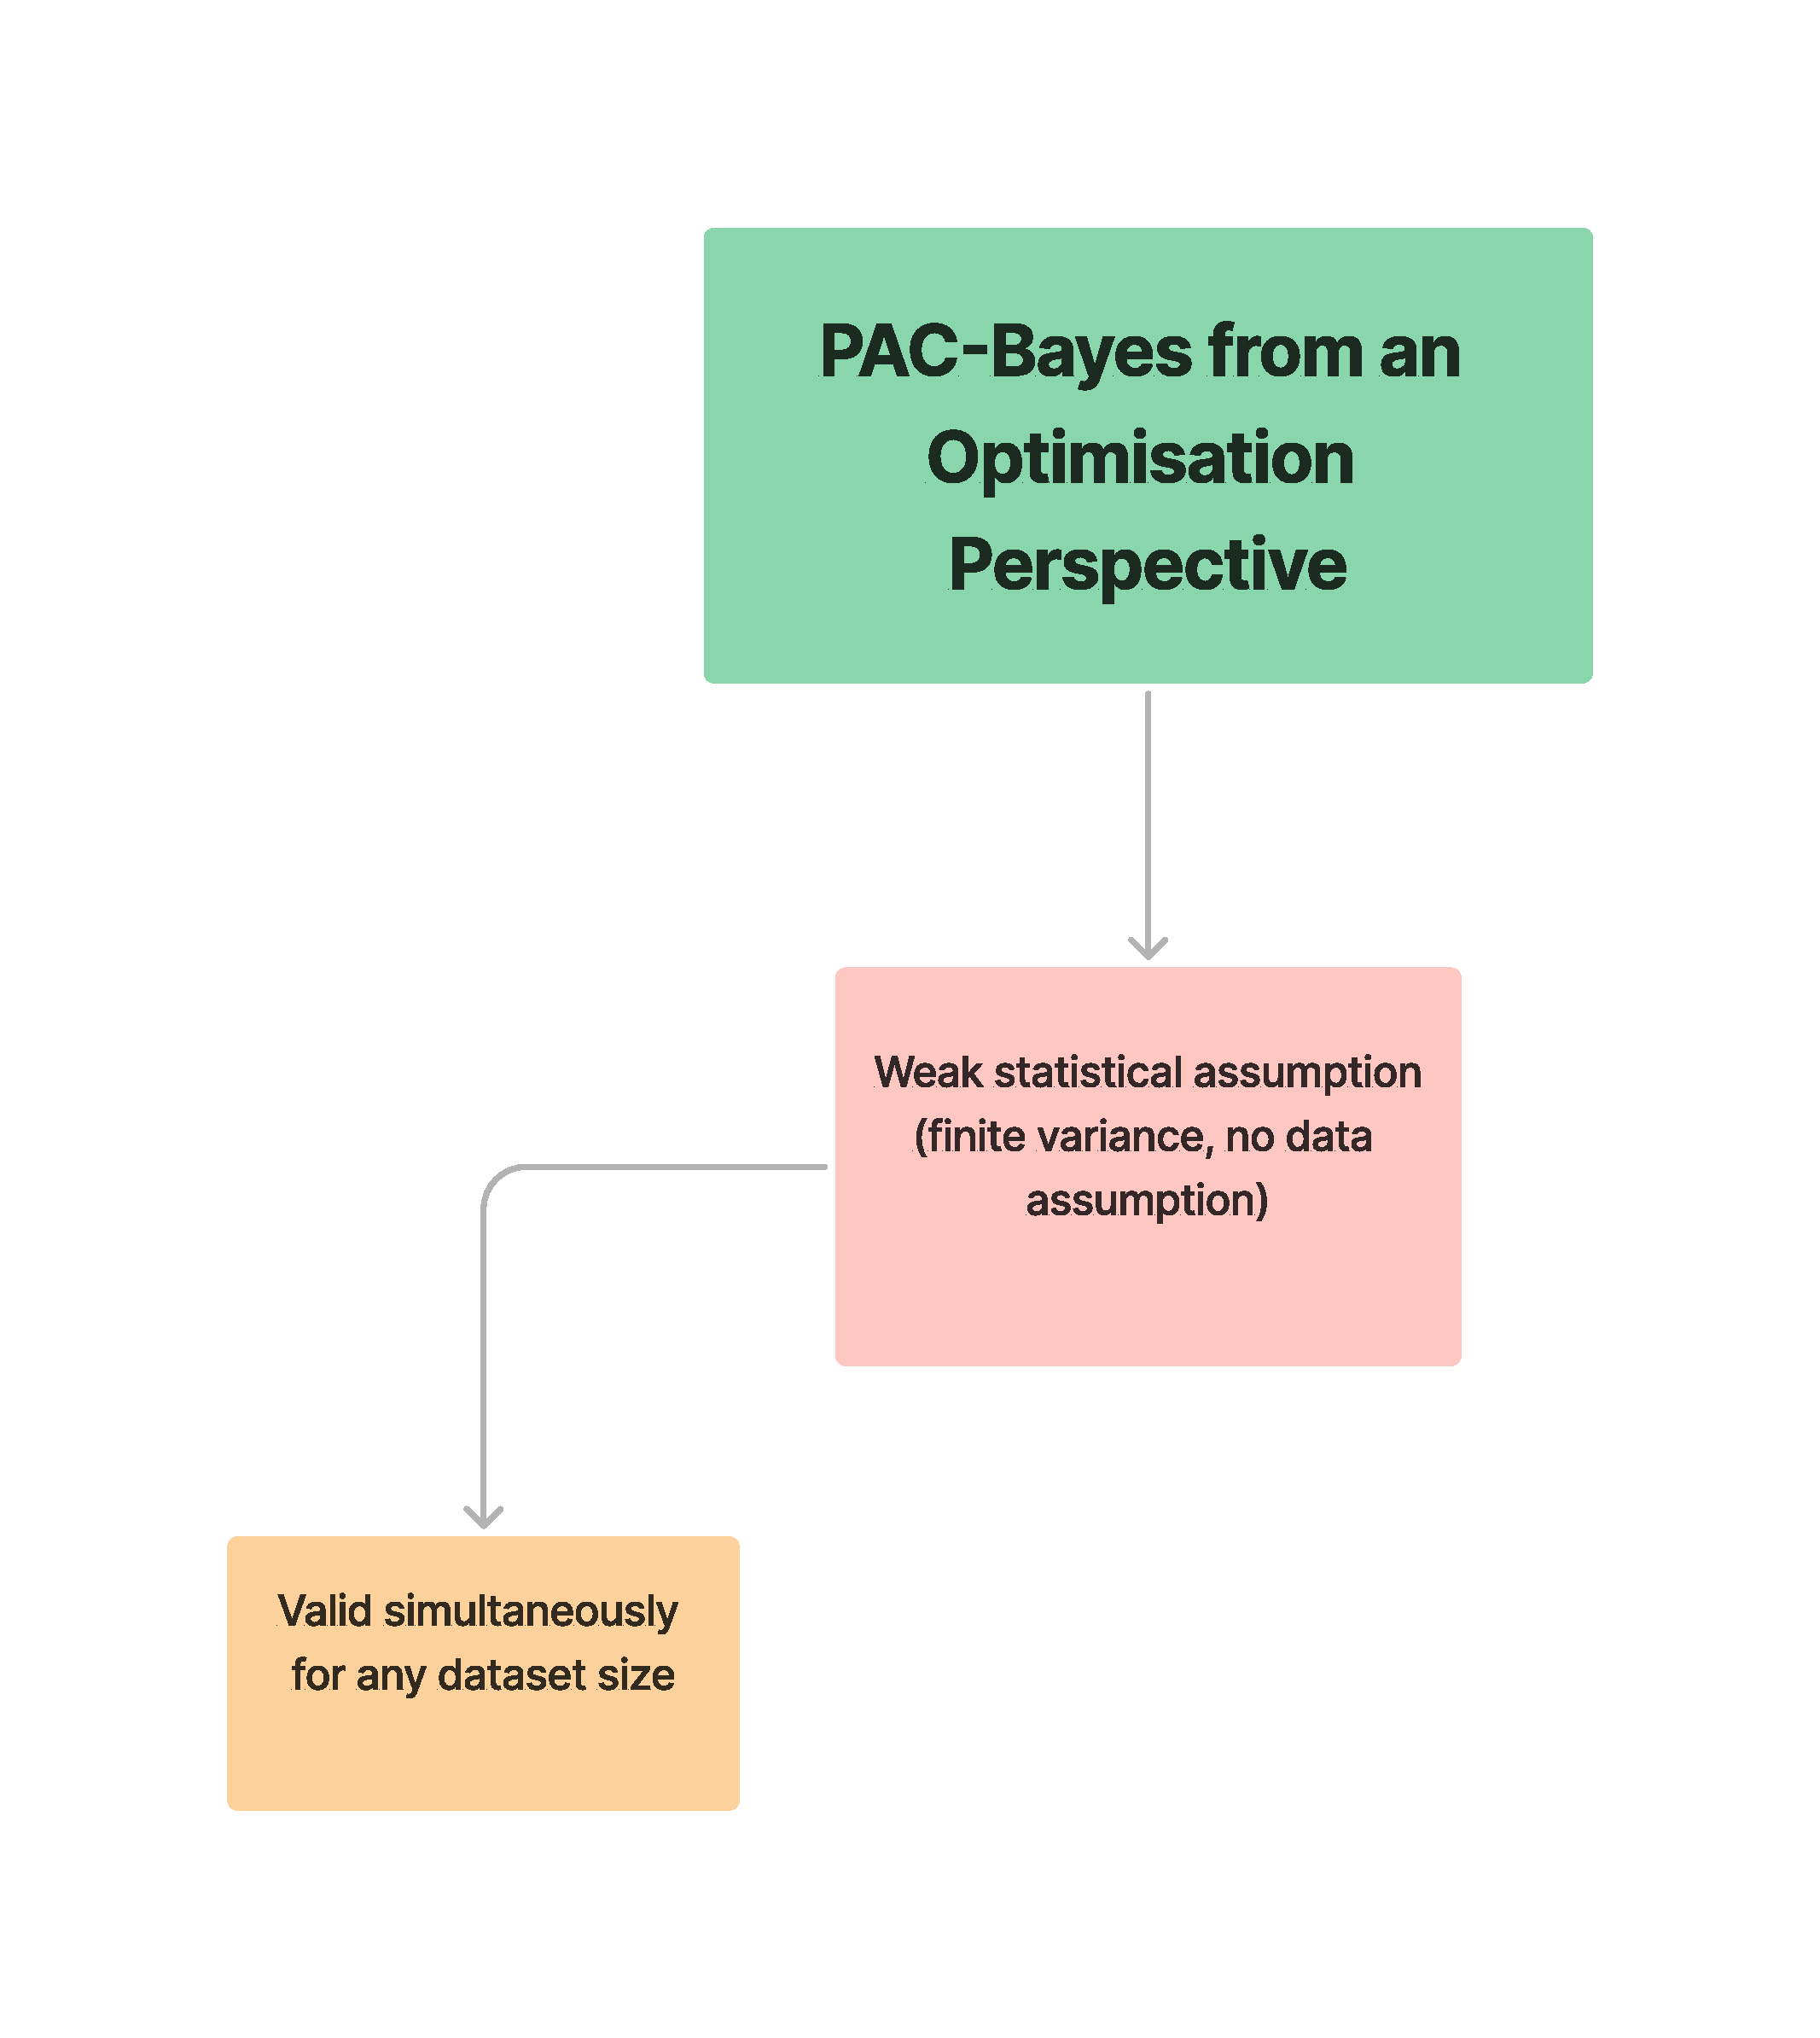
\includegraphics[scale=0.14]{diagram-chap-2.pdf}
  \end{figure}
\end{xframe}

%Detail the main supermartingale bounds for batch learning

\section{Mitigating Initialisation Impact by Real-Time Control: Online PAC- Bayes Learning}

\begin{xframe}{Mitigating Initialisation Impact: Online PAC- Bayes Learning}
    \begin{figure}
        \centering
        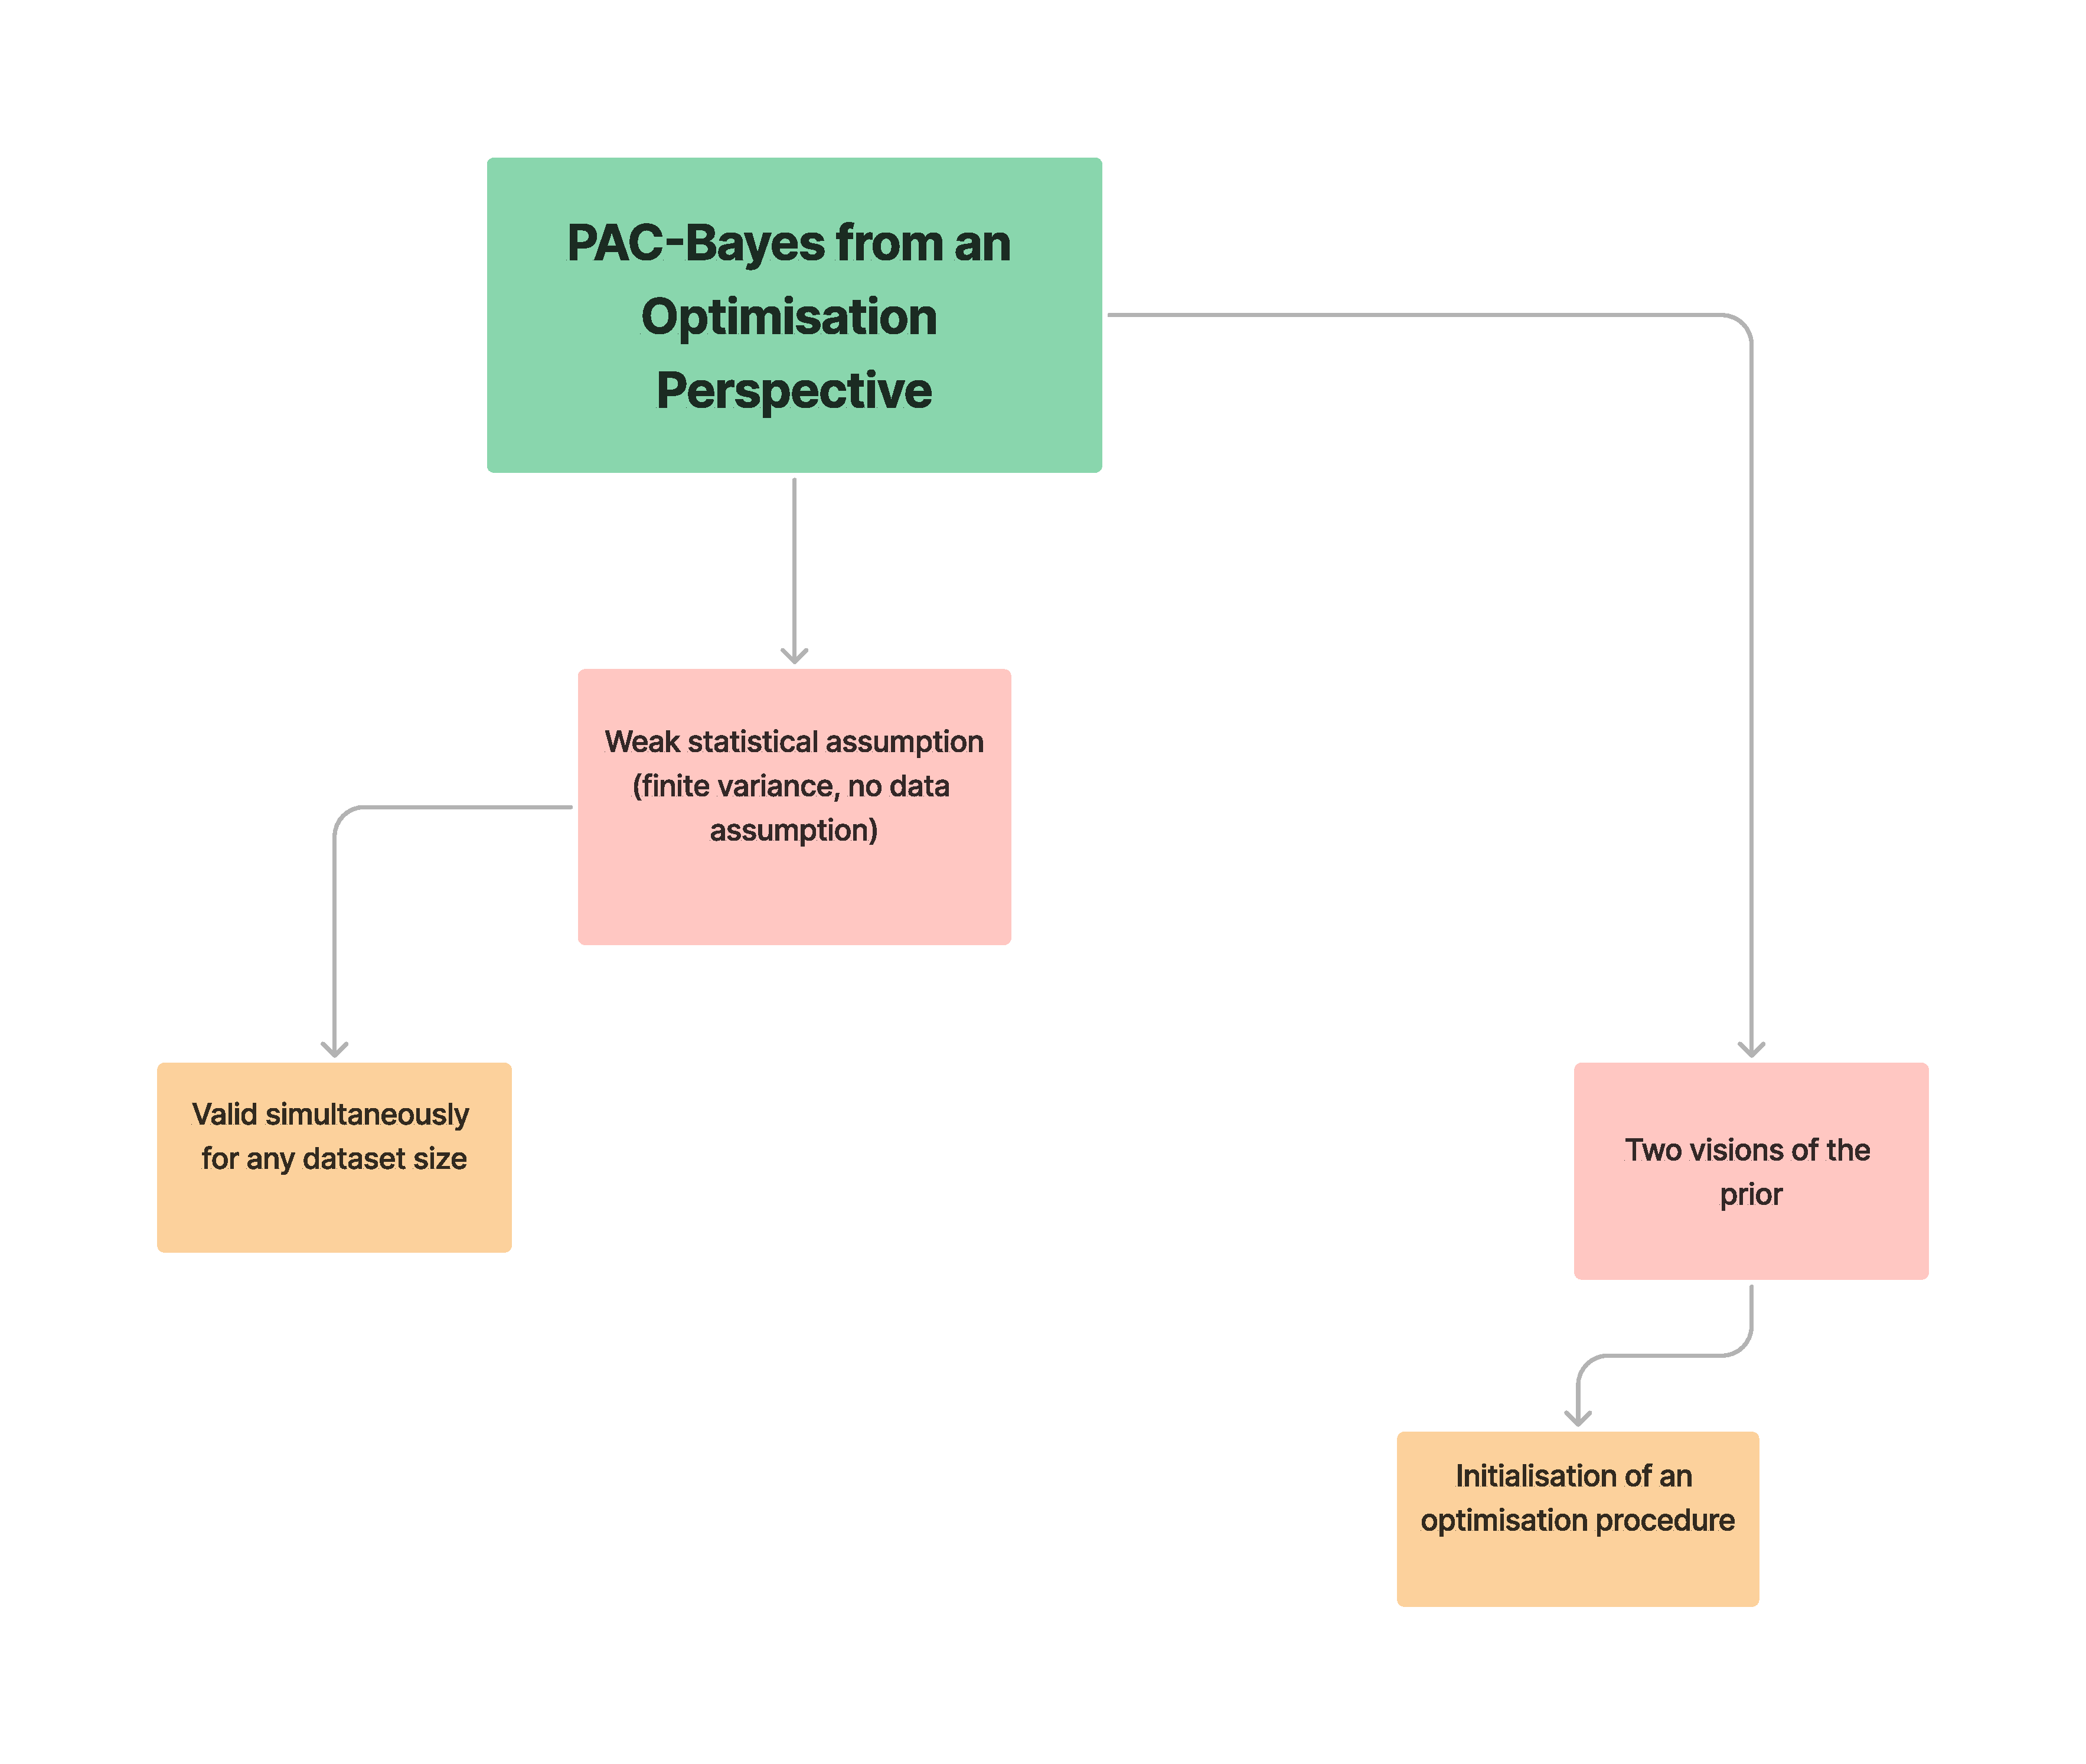
\includegraphics[scale=0.14]{diagram-chap-3.pdf}
    \end{figure}
  \end{xframe}

%Detail Online PAC-Bayes bounds alongside algorithmic results

\section{Mitigating Initialisation Impact through Flat Minima: Fast Rates for Small Gradients}

\begin{xframe}{Mitigating Initialisation Impact: Fast Rates for Small Gradients}
    \begin{figure}
        \centering
        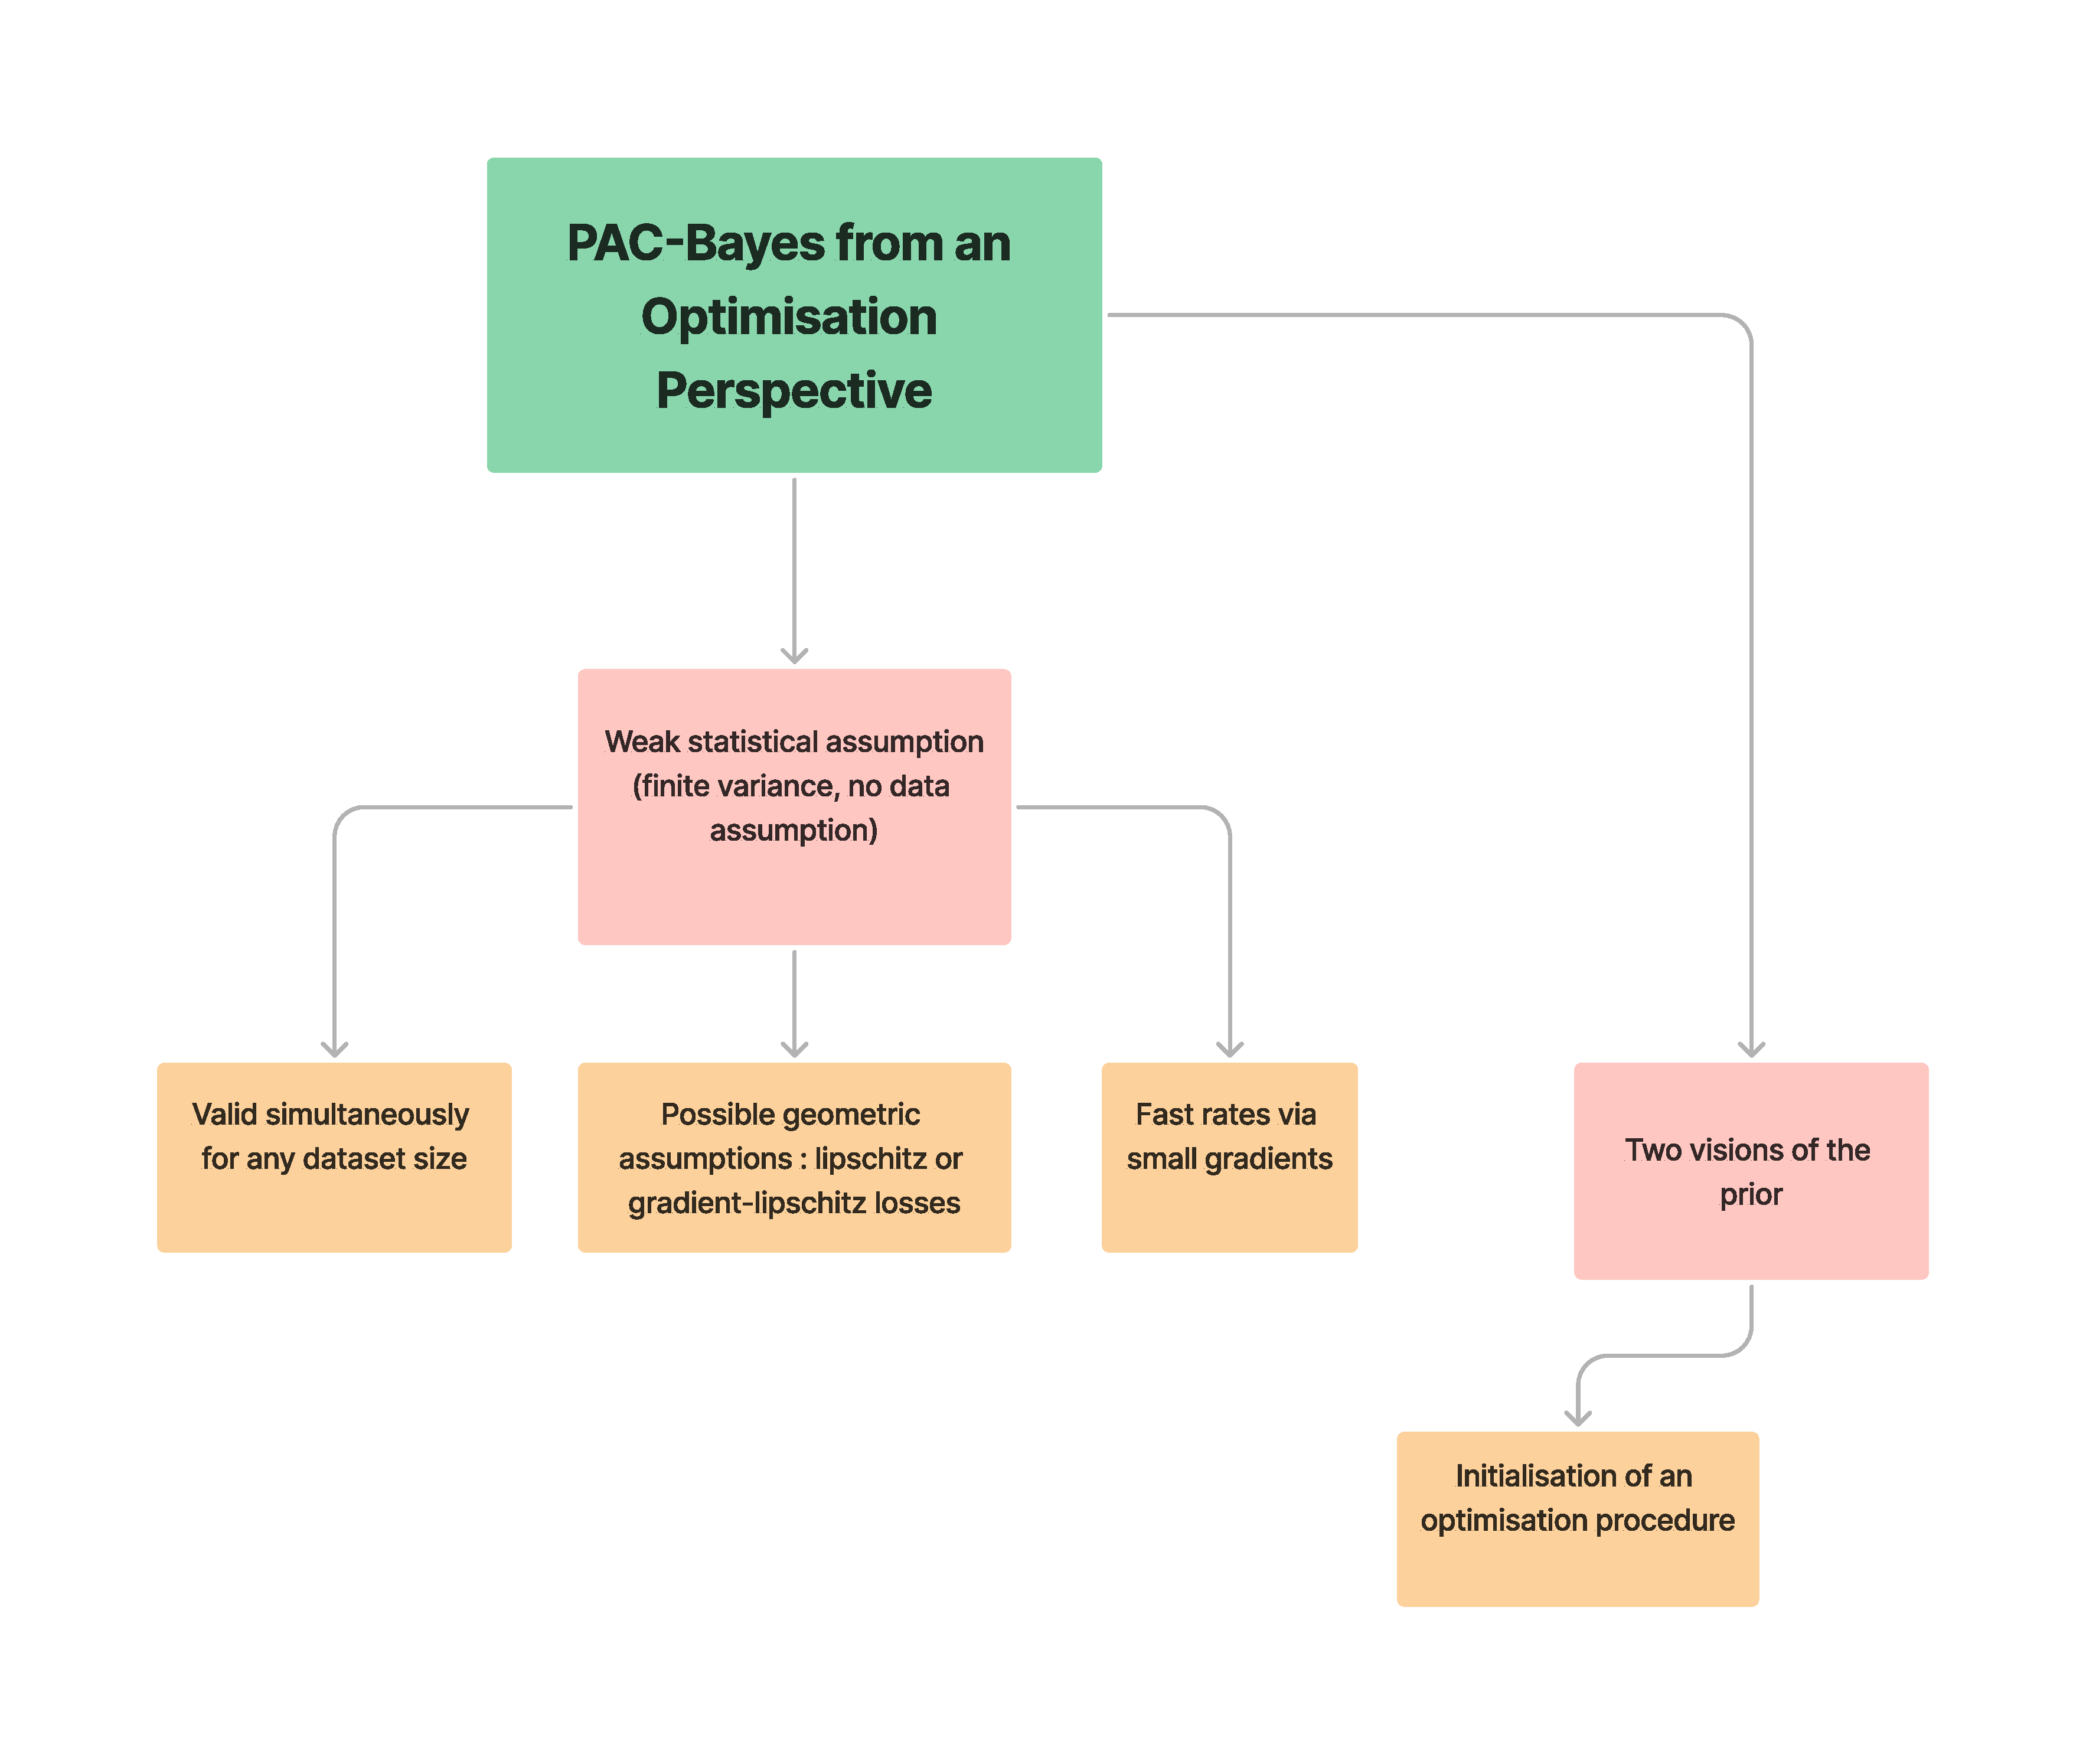
\includegraphics[scale=0.14]{diagram-chap-4.pdf}
    \end{figure}
  \end{xframe}

%Shrink this section
\begin{xframe}{Flat minimum}
    \textbf{What is a flat minimum?}
    \\
    \uncover<2->{\blue{A minimum such that its neighbourhood nearly minimises the loss.}
    \vspace{1cm}
    \begin{figure}
        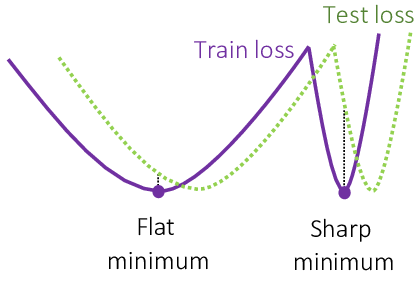
\includegraphics[scale= 0.5]{figures/flat-minima.png} 
    \end{figure}
{\tiny Image from \citet{liebenwein2021sparse}. }}
\end{xframe}


\begin{xframe}{Flat minima and generalisation are correlated!}
    \textbf{Correlations with generalisation recently emerged:}
    \vspace{0.5cm}
    \begin{xitemize}
        \item Flat minima of $\Riskhat_\S$.\\ PAC-Bayes based correlation measure : works for many datasets \citep{neyshabur2017explor,jiang2020fantastic,dziugaite2020search}
        \vspace{0.5cm}
        \item Flat minima of the adversarial loss in the context of adversarially robust learning. \citep{Stutz2021}
        \vspace{0.5cm}
        \item Flat minima implies generalisation for 2-layers nets \citep{wen2023sharpness}.
         
    \end{xitemize}
    \vspace{0.7cm}

    \uncover<2->{\blue{\textbf{Can we go beyond correlation or 2-layers net and obtain sound generalisation bounds involving directly flat minima?}}}
    
\end{xframe}

\begin{xframe}{Essential tools: Poincaré and log-Sobolev inequalities}
    \small{\green{Notation:} for any $\Q$, $\mathrm{H}^{1}(\Q) := \left\{ f\in \mathrm{L}^2(\Q)\cap \mathrm{D}_1(\mathbb{R}^d)\mid \|\nabla f\|\in \mathrm{L}^2(\Q) \right\}$}
    \begin{block}{\textbf{Poincaré}}
        $\Q$ is $\Poinc(c_{P})$ if for all  $f\in \mathrm{H}^{1}(\Q)$: 

        \[ \Var(f) \leq c_{P}(\Q) \EE_{h\sim \Q}\left[ \|\nabla f (h)\|^2 \right],  \]
  
    \end{block}

    \begin{block}{\bf Log-Sobolev}
        $\Q$ is $\Lsob(c_{LS})$ if for all function $f\in \mathrm{H}^{1}(\Q)$:

        \[ \EE_{h\sim\Q}\LB f^2(h)\log\LP \frac{f^2(h)}{\mathbb{E}_{h\sim\Q}\LB f^2(h)\RB}\RP \RB \leq c_{LS}(\Q) \EE_{h\sim \Q}\left[ \|\nabla f (h)\|^2 \right],  \]
    \end{block}
    \vspace{0.5cm}
    \uncover<2->{\textbf{Gaussian distributions and Gibbs posteriors are \Poinc \, and \Lsob!}}

\end{xframe}


\begin{xframe}{Fast-rate generalisation bounds for flat minima (1)}
  \small{\green{Notation:} $\Err(\ell,\Q,\z):= \EE_{h\sim\Q}[\ell(h,\z)]$}
    \vspace{1cm}
    \begin{block}{\textbf{Assumption}}
    $\Q\in\Mcal(\Hcal)$ is \emph{quadratically self-bounded} \wrt $\ell$ and  $C>0$ (namely $\texttt{QSB}(\ell,C)$) if
    \[ \mathbb{E}_{\z\sim \D}\LB \Err(\ell,\Q,\z)^2 \RB \leq C \Risk_\D(\Q) \LP = C\mathbb{E}_{\z\sim \D}\LB \Err(\ell,\Q,\z) \RB \RP   \]
    \end{block}
    \vspace{0.7cm}
    \begin{xitemize}
        \item QSB intricates $\D\in\Mcal(\Zcal)$ with $\Q \in \Mcal(\H)$
        \vspace{0.2cm}
        \item Satisfied if $\ell\in [0,K]$ with $C=K$.
        \vspace{0.2cm}
        \item \texttt{QSB} quantifies the 'flatness' of the post-training minima reached by $\Q$.
    \end{xitemize}
    
    
\end{xframe}

\begin{xframe}{Is the QSB assumption verified in practice?}
    \red{\textbf{QSB holds for 3-layer neural nets trained on MNIST (black curve)!}}
  \begin{figure}
      \centering
      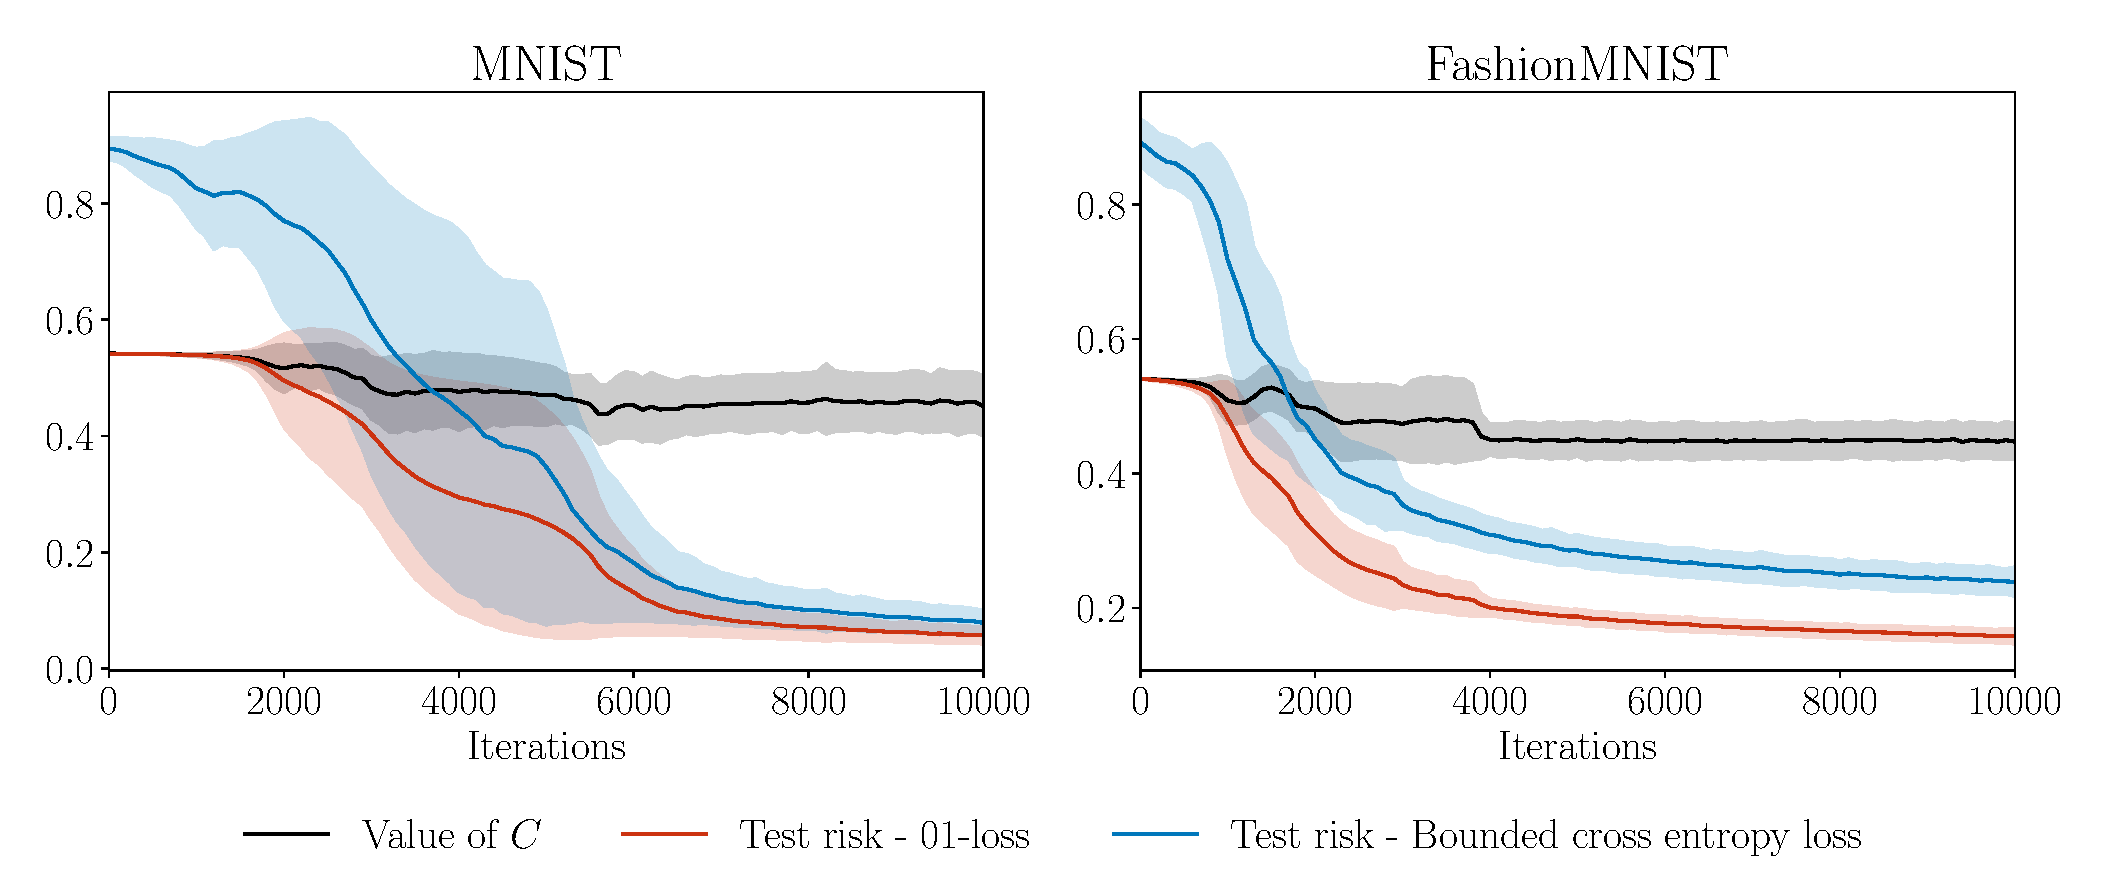
\includegraphics[scale=0.4]{result-flat-minima.pdf}
  \end{figure}
\end{xframe}

\begin{xframe}{Fast-rate generalisation bounds via flat minima (2)}
  \begin{block}{\bf Theorem}
      For any $C>0$, data-free prior $\P$, with probability at least $1-\delta$ for any $m>0$, and $\Q$ being $\Poinc(c_P)$, $\texttt{QSB}(\ell,C)$,
      \begin{align*}
      \Risk_{\D}(\Q) \leq  2\hat{\Risk}_{\S}(\Q) + 2C\frac{KL(\Q,\P) +\log(1/\delta)}{ m}  
       + \frac{1}{C} c_{P}(\Q)\EE_{\z\sim\D} \LB \EE_{h\sim \Q}\LP \|\nabla_h \ell(h,\z)\|^2 \RP \RB .
    \end{align*}
  \end{block}

  \uncover<2->{ \begin{block}{\bf \red{If $\D$ is also \Poinc:}}
       With more minor technical assumptions, for any $\Q$ being $\Poinc(c_P)$ with $\Risk_\D(\Q)\leq C$:
    \begin{multline*}
      \Risk_{\D}(\Q) \leq 2 \hat{\Risk}_{\S}(\Q) + 2C\frac{KL(\Q,\P) +\log(1/\delta)}{  m} \\
      + \frac{1}{C}\LP c_{P}(\Q)\EE_{\z\sim\D} \LB \EE_{h\sim \Q}\LP \|\nabla_h \ell(h,\z)\|^2 \RP \RB  + c_{P}(\D)\EE_{\z\sim\D} \LP \left\|\EE_{h\sim\Q}[\nabla_z \ell(h,\z)] \right\|^2\RP  \RP.
    \end{multline*} 
  \end{block}} 
\end{xframe}


\begin{xframe}{Fully empirical fast rate}
    \textbf{Current drawback: bounds are not empirical.}
    \vspace{0.3cm}
    
    \uncover<2->{\green{\textbf{Solution: $\mathcal{C}^2$ gradient-lipschitz losses!}}
    
    \begin{block}{\bf Theorem}
        For any $C_1,C_2,c>0$, with probability at least $1-\delta$, for any $m>0$, $\Q$ being $\Poinc(c_P)$ with constant $c$, $\texttt{QSB}(\ell,C_1)$, $\texttt{QSB}\LP\|\nabla_h \ell\|^2,C_2\RP$, 

    \begin{align*}
      \Risk_{\D}(\Q) \leq &\; 2 \hat{\Risk}_{\S}(\Q) + \mathcal{O}\left( \EE_{h\sim \Q}\LB \frac{1}{m}\sum_{i=1}^m \|\nabla_h\ell(h,\z_i)\|^2 \RB  + \frac{\KL(\Q,\P) +\log(1/\delta)}{m}\right).
    \end{align*}
    \end{block}
    }
\end{xframe}

\begin{xframe}{Take-home messages}
    \vspace{1.5cm}
    \Large{
        If $\Q$ satisfies either
        \begin{enumerate}
            \item Flat minima for $\Riskhat_\S$ and $\Risk_\D$, 
            \item if $\ell$ gradient-lipschitz, flat minima for $\Riskhat_\S$ and empirical gradient norms, 
        \end{enumerate}
    \textbf{then $\Q$ generalises well!}
    }
\end{xframe}

\begin{xframe}{Gibbs posteriors}
    \textbf{Current limitation: with Poincaré posteriors, KL is uncontrolled.}
    \vspace{0.3cm}
    
    \uncover<2->{\green{\textbf{Solution: consider Gibbs posterior with log-Sobolev priors!}}
    
    \begin{block}{\bf Definition}
       $\P_{-\gamma \hat{\Risk}_\S}$ is the Gibbs posterior \wrt prior $\P$ with \emph{inverse temperature} $\gamma>0$  if  $$d\P_{-\gamma \hat{\Risk}_\S}(h)\propto \exp\LP - \gamma \hat{\Risk}_\S(h) \RP dP(h)$$. 
    \end{block}
    \vspace{0.3cm}
    \begin{block}{\bf Why focus on those?}
        \begin{xitemize}
        \item Minimise Catoni's bound \citep[Theorem 4.1]{AlquierRidgwayChopin2016}
        \item if $\P$ \Lsob (+ technical assumptions) and $\ell= \ell_1 + \ell_2$ ($\ell_1$ convex, twice differentiable, $\ell_2$ bounded) then $\P_{-\gamma \hat{\Risk}_\S}$ is $\Lsob$.
    \end{xitemize}
    \end{block}
    }
\end{xframe}

\begin{xframe}{Understanding Gibbs posteriors through flat minima}

    \begin{block}{\bf Theorem}
        For any $C>0$, any $\gamma>0$, any prior $\P$ $\Lsob(c_{LS})$ (+ technical assumptions), if $\ell=\ell_1+\ell_2$ (as above), then with probability at least $1-\delta$, for any $m>0$, $\Q$ being $\texttt{QSB}(\ell,C)$:

  \begin{multline*}
    \Risk_{\D}(\P_{-\gamma \hat{\Risk}_\S})  \leq 2  \hat{\Risk}_{\S}(\P_{-\gamma \hat{\Risk}_\S}) + \\
    \mathcal{O}\LP C\frac{\gamma^2\EE_{h\sim \P_{-\gamma \hat{\Risk}_\S}}\LB \|\nabla_h \hat{\Risk}_\S(h) \|^2 \RB+\log(1/\delta)}{ m} + \frac{ 1 }{C} \EE_{\z\sim\D} \LB \EE_{h\sim \P_{-\gamma \hat{\Risk}_\S}}\LP \|\nabla_h \ell(h,\z)\|^2 \RP \RB \RP.
  \end{multline*} 
    \end{block}
    \uncover<2->{\bf KL small if a flat minima on $\Riskhat_\S$ is reached: \\\blue{$\rightarrow$ Flat minima fully explain generalisation here!}}
\end{xframe}

\begin{xframe}{Take-home messages}
    \vspace{1.5cm}
    \Large{
        \begin{enumerate}
            \item Gibbs posterior generalises well if they reach a flat minima on both $\Riskhat_\S$ and $\Risk_\D$.
            \item Flatness of the minimum on $\Riskhat_\S$ controls the expansion of KL.
        \end{enumerate}
    }
\end{xframe}

\begin{xframe}{Result for deterministic predictors}
    \Large 
    \vspace{2.5cm}
    \red{\textbf{Drawback: results hold for probabilistic predictors}}
    
    \vspace{0.3cm}
    \uncover<2->{\green{\textbf{Answer: Exploit the 2-Wasserstein distance to obtain guarantees valid for deterministic predictors (Diracs) }}}

    
\end{xframe}

\begin{xframe}{Convergence guarantees for non-convex SGD}

    \begin{block}{\bf Key tool: a novel change of measure inequality}
        For any $f$ gradient lipschitz, any $\P,\Q$:

         \[ \mathbb{E}_{h\sim \Q}[f(h)] \leq \frac{G}{2}W_2^2(Q,P) + \mathbb{E}_{h\sim \P}[f(h)] +D \mathbb{E}_{h\sim\Q}[\|\nabla f (h)\|].  \]

         \textbf{NB:} a variant of this formula with a KL is attainable if $\Q<<\P$ and $\P$ is $\Lsob$ !
    \end{block}

    \begin{block}{\bf Assumption}
        \begin{xitemize}
            \item Gradient-lipschitz loss.
            \item $\P \propto exp(-V(h))dh$
        \end{xitemize}
    \end{block}
\end{xframe}

\begin{xframe}{Result}
\vspace{1cm}
\begin{block}{\bf Theorem}
    Let $\delta\in(0,1)$ and $P\in\Mcal(\Hcal)$ a data-free prior.
Assume $\Hcal$ has a finite diameter $D>0$, $\ell\geq 0$ and that for any $m$, the generalisation gap $\Delta_{\S_m}$ is $G$ gradient-Lipschitz.
Assume that $\mathbb{E}_{h\sim\P}\Ebb_{\z\sim\D}[\ell(h,z)^2] \leq \sigma^2$, then the following holds with probability at least $1-\delta$, for any $m>0$ and any $\Q$:
\begin{align*}
    \Risk_D(\Q) \leq \hat{\Risk}_{\S_m}(\Q) + \frac{G}{2} W_2^2(\Q,\P) + \sqrt{\frac{2\sigma^2\log\LP \frac{1}{\delta} \RP}{m}} + D \mathbb{E}_{h\sim \Q}\LP \left\| \nabla_h \Risk_\D(h) - \nabla_h \hat{\Risk}_{\S_m}(h) \right\| \RP
\end{align*}
\end{block}
 
\end{xframe}

\begin{xframe}{Conclusion}
    \vspace{1cm}
    \Large
    \begin{xitemize}
        \item We mathematically quantify the impact of flat minima in generalisation: momentum in Catoni's bound!
        \item The \texttt{QSB} condition is verified on basic neural nets (classification) with constant $C$ sharper than 1! 
        \item A crucial future lead: understanding why optimisation procedures on deep nets lead to flat minima: \textbf{here we are only able to explain why flat minima generalise well, not how we reach them.}
    \end{xitemize}

    Full paper available at \url{https://arxiv.org/abs/2402.08508}
    
\end{xframe}

\section{Wasserstein PAC-Bayes: Exploiting Optimisation to Explain Generalisation}

\begin{xframe}{Wasserstein PAC-Bayes: From Optimisation to Generalisation}
    \begin{figure}
        \centering
        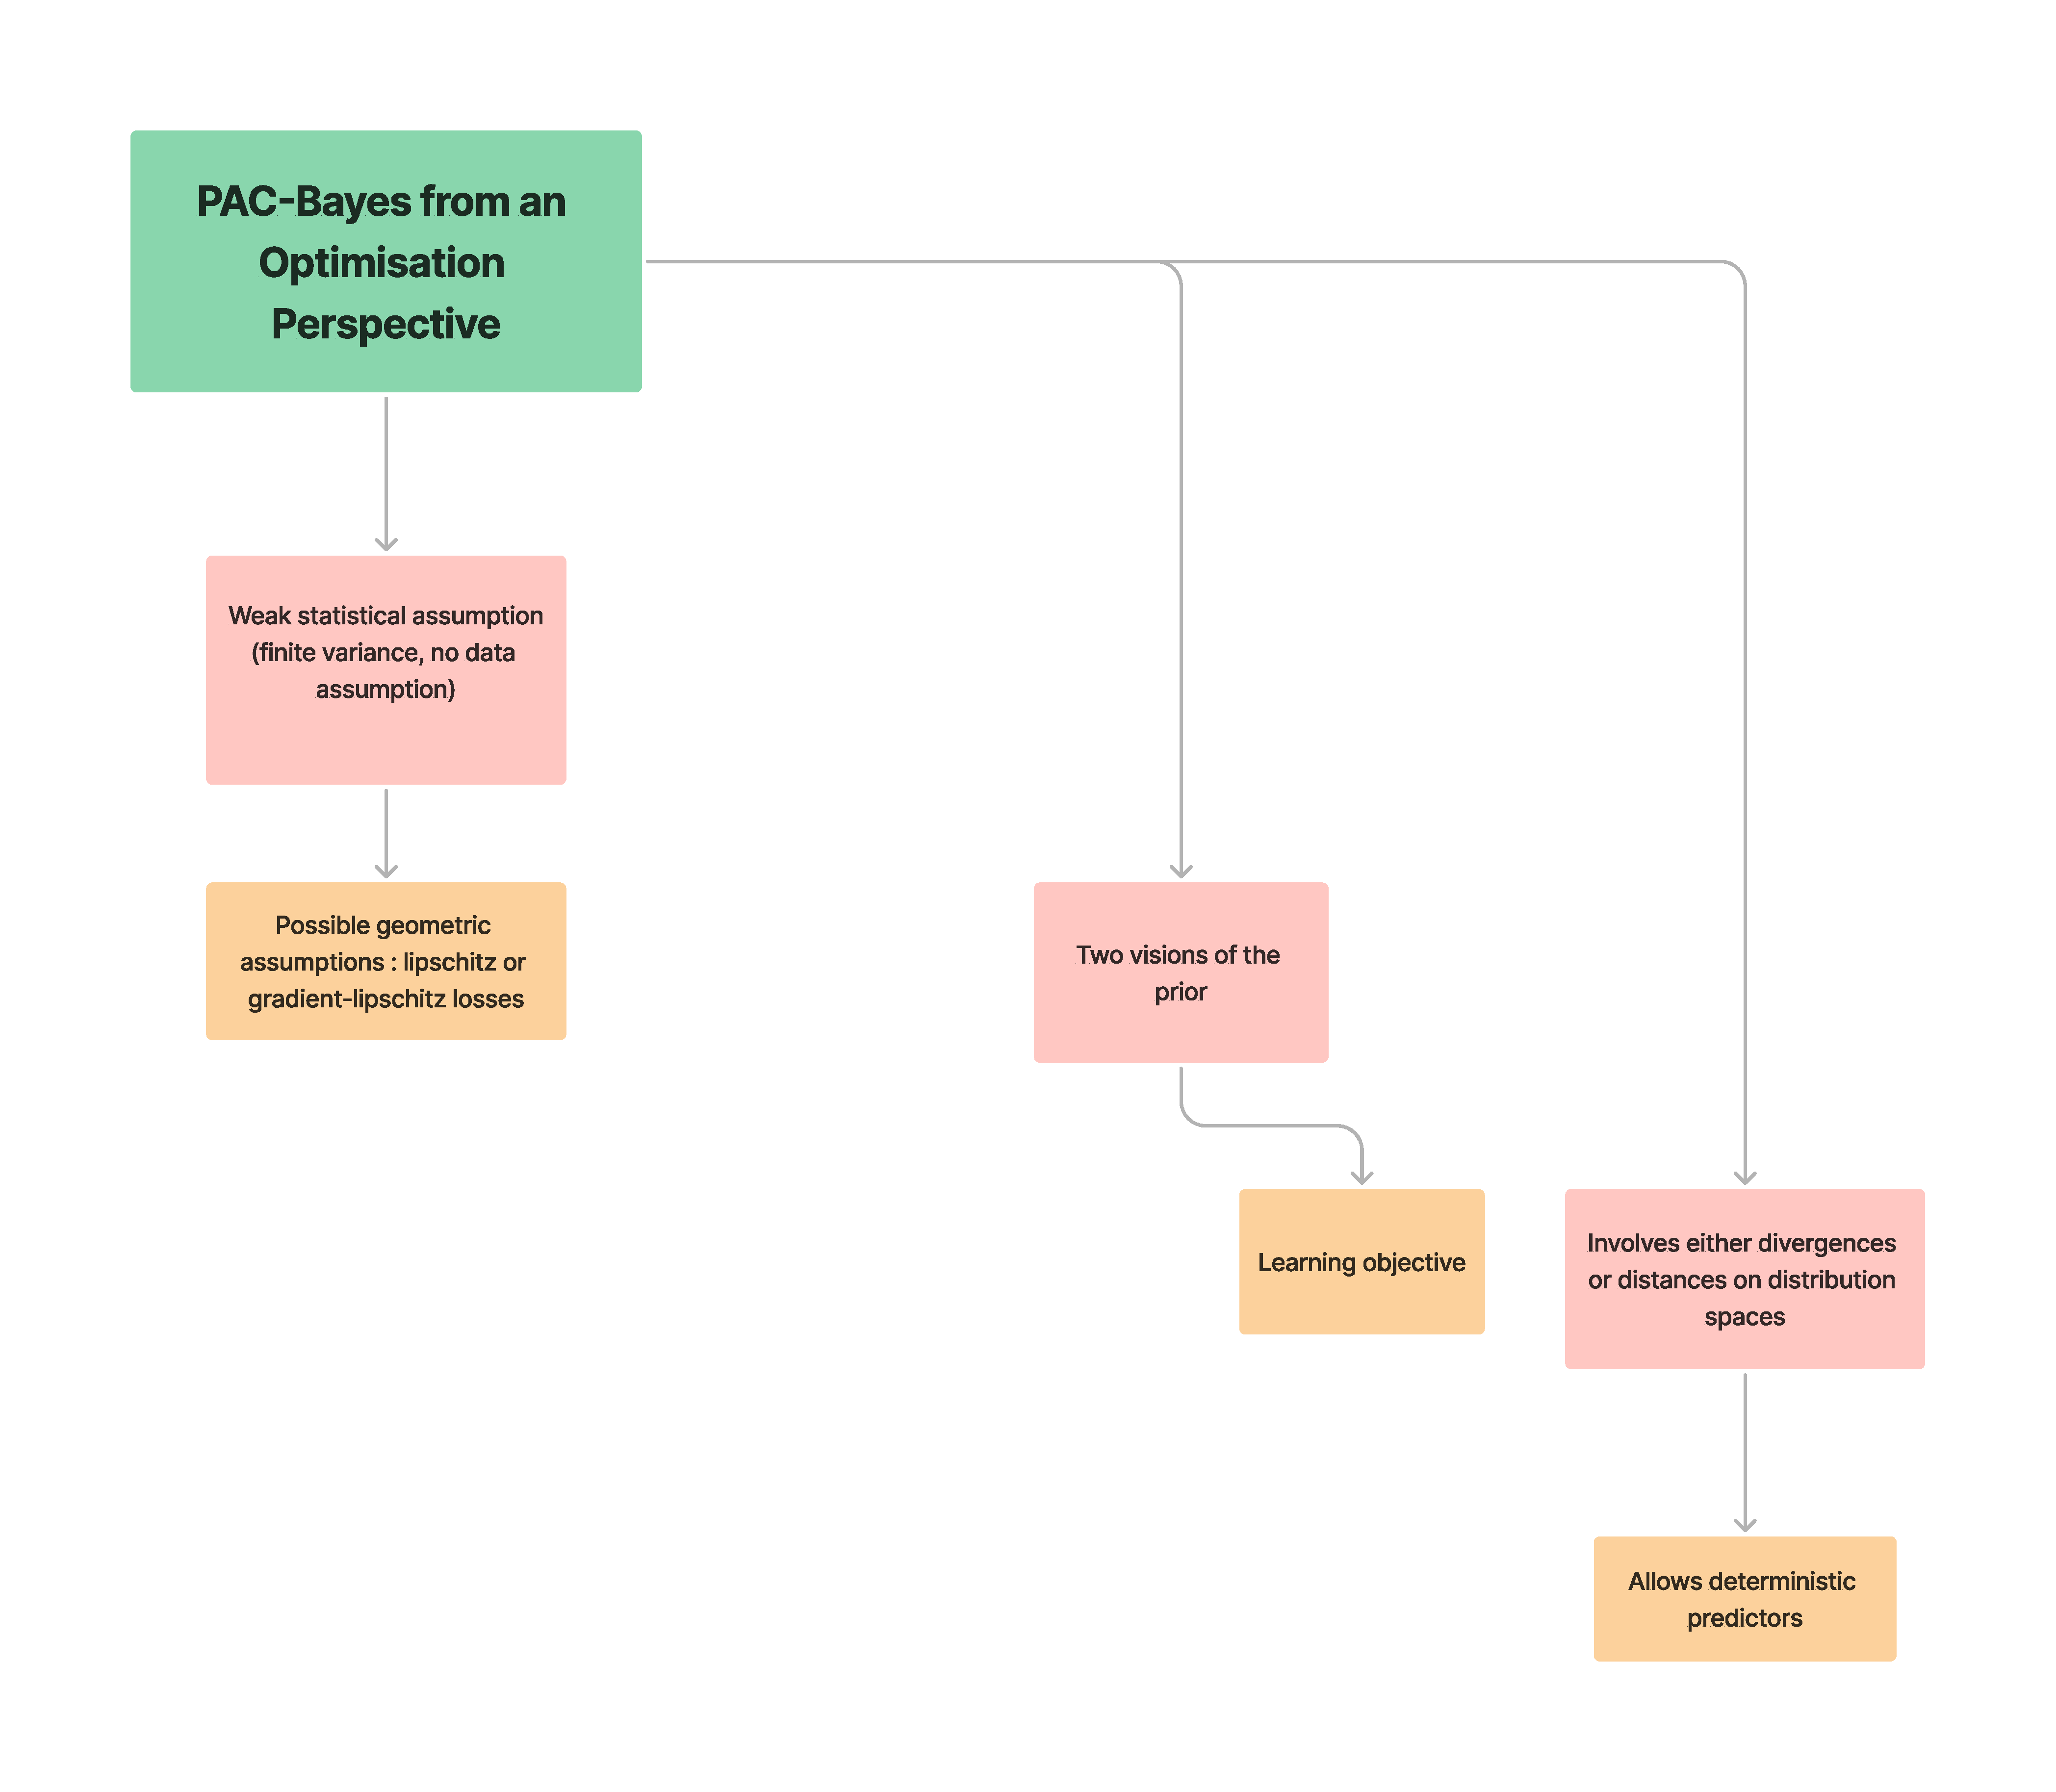
\includegraphics[scale=0.14]{diagram-chap-5.pdf}
    \end{figure}
  \end{xframe}

%Explain the broad ideas, put only few bounds

\section{Wasserstein PAC-Bayes in Practice: Generalisation-Driven Algorithms for Deterministic Predictors}

\begin{xframe}{Wasserstein PAC-Bayes in Practice Allows Dirac Predictors}
    \begin{figure}
        \centering
        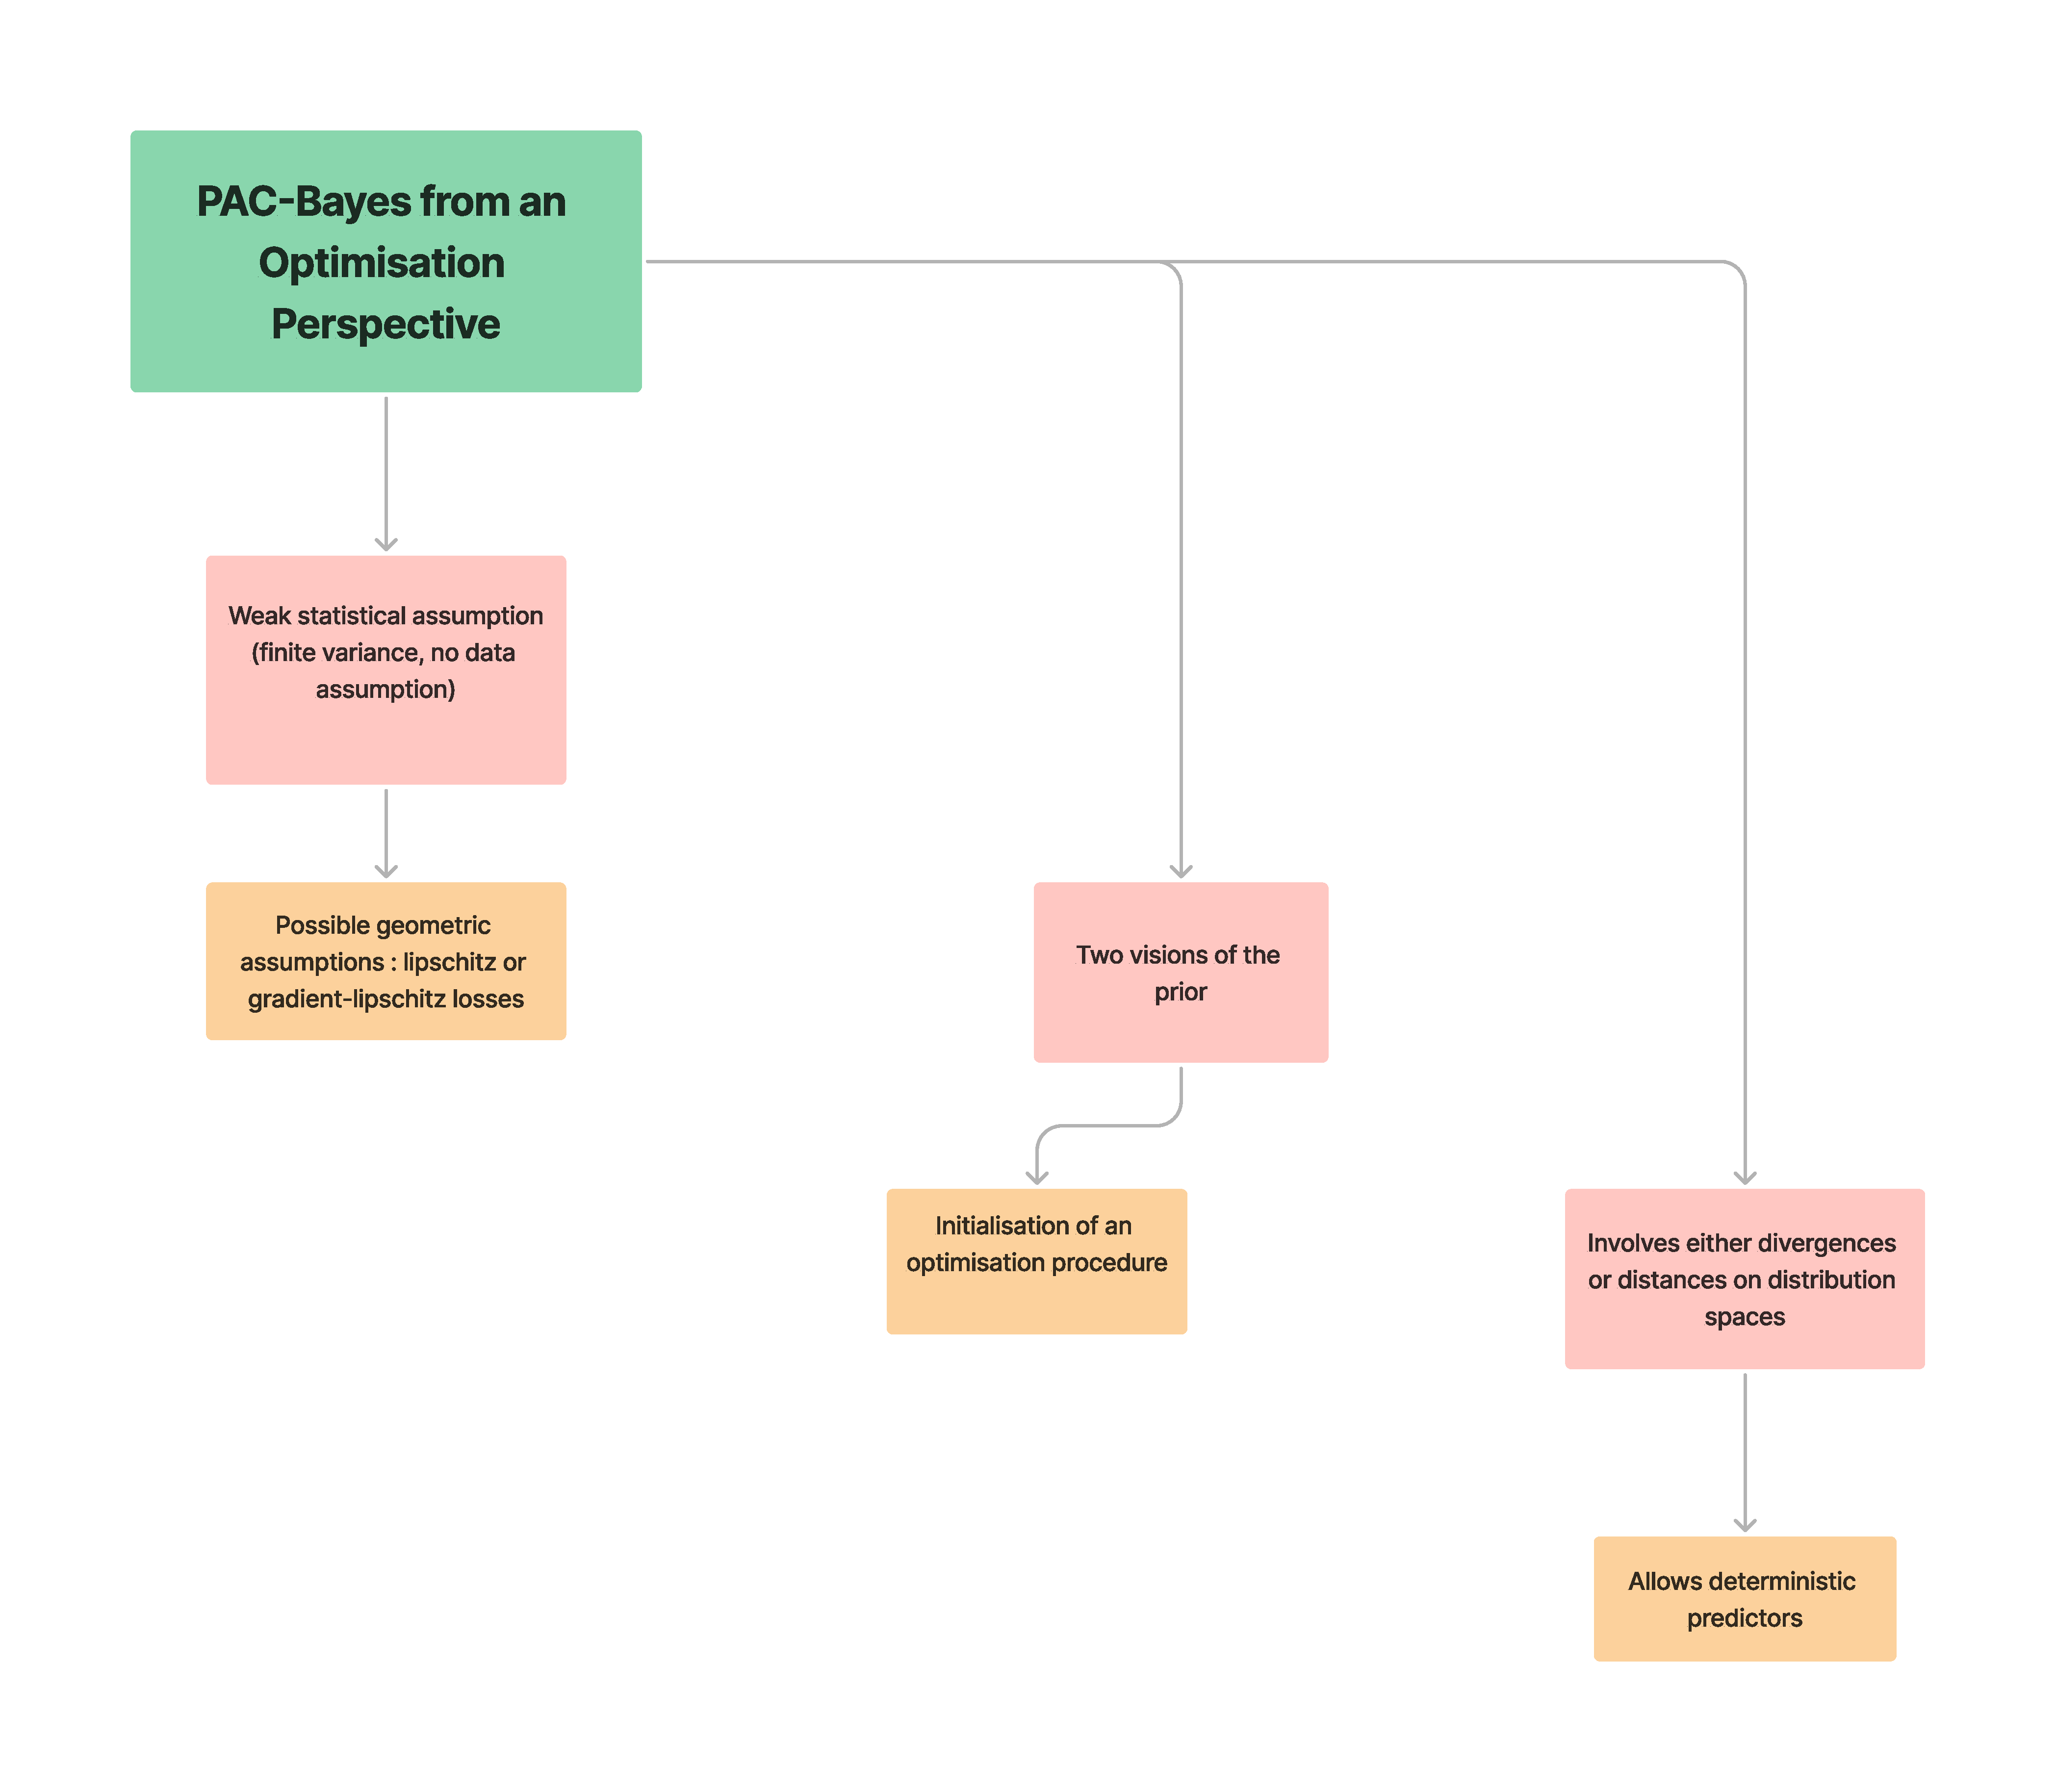
\includegraphics[scale=0.14]{diagram-chap-6.pdf}
    \end{figure}
  \end{xframe}

%Insist on algorithms

\section{Conclusion}



%%%%%%%%%%%%%%%%%%%%%%%%%%%%%%%%%%%%%%%%%%%%%%%%%%%%%%%%%%%%%%%%%%%%%%%%%%%%%%%


%%%%%%%%%%%%%%%%%%%%%%%%%%%%%%%%%%%%%%%%%%%%%%%%%%%%%%%%%%%%%%%%%%%%%%%%%%%%%%%



%%%%%%%%%%%%%%%%%%%%%%%%%%%%%%%%%%%%%%%%%%%%%%%%%%%%%%%%%%%%%%%%%%%%%%%%%%%%%%%

\appendix

\begin{frame}[t,noframenumbering,allowframebreaks]
  \frametitle{References}
  \printbibliography[title={References}]
 \end{frame}

\begin{xtitle}

\vspace{2.0cm}
{\bf Thank you for your attention!}\\

\end{xtitle}

%%%%%%%%%%%%%%%%%%%%%%%%%%%%%%%%%%%%%%%%%%%%%%%%%%%%%%%%%%%%%%%%%%%%%%%%%%%%%%%
 
\end{document}